\documentclass[12pt, a4paper]{report}

\input{preamble}

\begin{document}

\begin{titlepage}
    \centering
    \vspace*{2cm}

    {\Huge\bfseries Math 132\\[0.3cm]}
    {\Large Differential Topology}\\[1.5cm]

    {\large\itshape Lecture Notes}\\[2cm]

    {\normalsize
    \textbf{Textbook:}\\[0.3cm]
    Victor Guillemin \& Alan Pollack, \textit{Differential Topology} (1974)
    }\\[2cm]

    {\normalsize
    \textbf{Topics:}\\[0.3cm]
    \begin{enumerate}[label=(\roman*)]
        \item Smooth manifolds and smooth maps
        \item Transversality and intersection theory
        \item Oriented intersection theory and applications
    \end{enumerate}
    }\vspace{2cm}

    {\small Spring 2026 \quad$\cdot$\quad Harvard University}

    \vfill
\end{titlepage}


\tableofcontents
\newpage

\chapter{Smooth Manifolds}
% lecture01.tex — Smooth Manifolds

\section{Smooth Manifolds}

$\R^k$: $k$-dimensional Euclidean space, i.e.\ a point $x \in \R^k$ is a $k$-tuple $x = (x_1, \ldots, x_k)$ of real numbers.

\begin{definition}{Smooth Map (Open Sets)}{smooth-map-open}
    For open sets $U \subset \R^k$ and $V \subset \R^\ell$, a map $f \colon U \to V$ is called \emph{smooth} (or $C^\infty$) if all the partial derivatives $\frac{\partial^n f}{\partial x_{i_1} \cdots \partial x_{i_n}}$ exist and are continuous.
\end{definition}

More generally, for arbitrary subsets $X \subset \R^k$ and $Y \subset \R^\ell$:

\begin{definition}{Smooth Map (Arbitrary Subsets)}{smooth-map-arbitrary}
    A map $f \colon X \to Y$ is called \emph{smooth} if for each $x \in X$ there exists an open $U \subset \R^k$ containing $x$ and a smooth map $F \colon U \to \R^\ell$ such that $F = f$ on $U \cap X$.
\end{definition}

\begin{center}
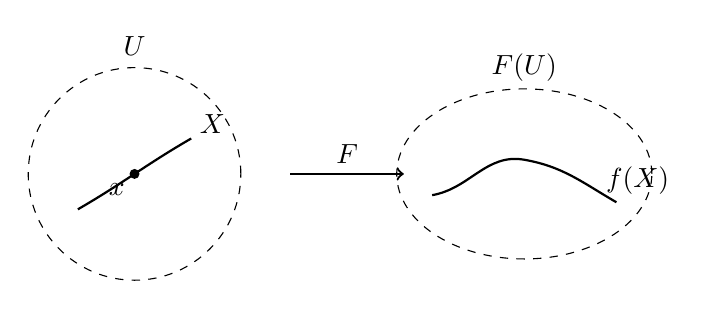
\begin{tikzpicture}[scale=0.9]
    % Left: U containing X with point x
    \draw[dashed] (0,0) circle (1.5);
    \node at (0,1.8) {$U$};
    \draw[thick] (-0.8,-0.5) to[out=30,in=210] (0.8,0.5);
    \node at (1.1,0.7) {$X$};
    \fill (0,0) circle (2pt) node[below left] {$x$};
    % Arrow
    \draw[->,thick] (2.2,0) -- (3.8,0) node[midway,above] {$F$};
    % Right: F(U) containing f(X)
    \draw[dashed] (5.5,0) ellipse (1.8 and 1.2);
    \node at (5.5,1.5) {$F(U)$};
    \draw[thick] (4.2,-0.3) to[out=10,in=170] (5.5,0.2) to[out=-10,in=150] (6.8,-0.4);
    \node at (7.1,-0.1) {$f(X)$};
\end{tikzpicture}
\end{center}

\begin{proposition}{Composition of Smooth Maps}{comp-smooth}
    If $f \colon X \to Y$ and $g \colon Y \to Z$ are smooth, then $g \circ f \colon X \to Z$ is also smooth. \quad (Easy exercise.)
\end{proposition}

\begin{definition}{Diffeomorphism}{diffeomorphism}
    A map $f \colon X \to Y$ is called a \emph{diffeomorphism} if it is bijective and both $f$ and $f^{-1}$ are smooth.
\end{definition}

\begin{remark}{Meta-definition: Differential Topology}{meta-def-diff-top}
    \emph{Differential topology} is the study of properties of ``spaces'' which are invariant under diffeomorphism.
\end{remark}

A particularly nice class of ``spaces'' is:

\begin{definition}{Smooth Manifold}{smooth-manifold}
    A subset $M \subset \R^k$ is called a \emph{smooth manifold of dimension $m$} (or simply a \emph{smooth $m$-manifold}) if it is locally diffeomorphic to $\R^m$, i.e.\ if each $x \in M$ has a neighborhood $W \cap M$ that is diffeomorphic to an open $U \subset \R^m$.

    A diffeomorphism $\phi \colon U \to W \cap M$ is called a \emph{parametrization} of the region $W \cap M$. The inverse diffeomorphism $\phi^{-1} \colon W \cap M \to U$ is called a \emph{coordinate system} on $W \cap M$.
\end{definition}

\begin{example}{The Unit Sphere}{unit-sphere}
    The unit sphere $S^2 = \{(x,y,z) \in \R^3 \mid x^2 + y^2 + z^2 = 1\}$ is a smooth 2-manifold (i.e.\ a smooth surface).

    For instance, the diffeomorphism
    \[
        (x,y) \mapsto (x, y, \sqrt{1 - x^2 - y^2}) \qquad (x^2 + y^2 < 1)
    \]
    parametrizes the region $z > 0$ of $S^2$.

    By interchanging the roles of $x, y, z$ and changing the signs, we obtain parametrizations of regions which cover $S^2$.

    More generally, $S^{n-1} = \{x \in \R^n \mid |x| = 1\}$ is a smooth $(n-1)$-manifold.
\end{example}

\begin{example}{Graph of $y = \sin(1/x)$}{sin-graph}
    $\{(x,y) \in \R^2 \mid x \neq 0,\; y = \sin(1/x)\}$ is a smooth 1-manifold.
\end{example}

\begin{center}
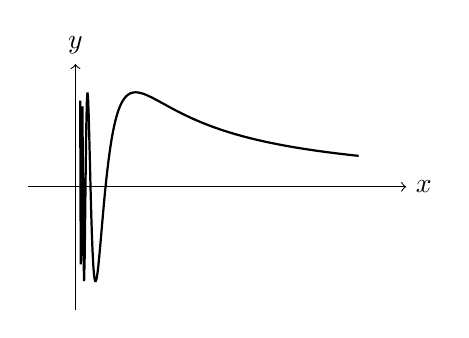
\begin{tikzpicture}[scale=1.2]
    \draw[->] (-0.5,0) -- (3.5,0) node[right] {$x$};
    \draw[->] (0,-1.3) -- (0,1.3) node[above] {$y$};
    \draw[thick,domain=0.05:3,samples=500] plot (\x, {sin(1/\x r)});
\end{tikzpicture}
\end{center}

\begin{remark}{Extrinsic vs.\ Intrinsic Definition}{extrinsic-intrinsic}
    Note that the definition of smooth manifolds we gave is ``extrinsic'' in that $M$ is embedded in $\R^k$. We can also give a better, ``intrinsic'' definition as follows.
\end{remark}

\begin{definition}{Topological Manifold}{topological-manifold}
    A Hausdorff, second countable topological space $M$ is called a \emph{topological $m$-manifold} if it is locally homeomorphic to $\R^m$.
\end{definition}

\begin{definition}{Coordinate Chart}{coordinate-chart}
    A \emph{coordinate chart} is a pair $(U, x)$ consisting of open $U \subset M$ and a homeomorphism $x \colon U \to \R^m$ onto its image.
\end{definition}

Two charts $(U, x)$ and $(V, y)$ on $M$ are \emph{smoothly related} if the transition function $y \circ x^{-1} \colon x(U \cap V) \to y(U \cap V)$ is a diffeomorphism.

An \emph{atlas} on $M$ is a collection $\mathcal{A} = \{(U_\alpha, x_\alpha)\}_{\alpha \in A}$ of smoothly related charts which cover $M$ (i.e.\ $\bigcup_{\alpha \in A} U_\alpha = M$).

A \emph{smooth structure} on $M$ is a maximal atlas. (Any atlas can be completed to a unique smooth structure.)

\begin{definition}{Smooth Manifold (Intrinsic)}{smooth-manifold-intrinsic}
    A \emph{smooth $m$-manifold} is a topological $m$-manifold equipped with a smooth structure.
\end{definition}


\chapter{Derivatives and Tangents}
% lecture02.tex — Derivatives and Tangents

\section{Derivatives and Tangents}

\begin{itemize}
    \item For any smooth map $f \colon U \to V$ where $U \subset \R^k$ and $V \subset \R^\ell$ are open, the \emph{derivative} at $x \in U$ is the linear map
    \[
        df_x \colon \R^k \to \R^\ell
    \]
    defined by the directional derivative
    \[
        df_x(h) = \lim_{t \to 0} \frac{f(x + th) - f(x)}{t}, \qquad h \in \R^k.
    \]
    It can be represented by the $\ell \times k$ Jacobian matrix $\left(\frac{\partial f_i}{\partial x_j}(x)\right)_{\substack{i=1,\ldots,\ell \\ j=1,\ldots,k}}$.

    (After translation, this is the best approximation of $f$ by a (nonhomogeneous) linear map, at $x$.)

    \item By chain rule, for any commutative triangle of smooth maps
    \[
    \begin{tikzcd}
        U \arrow[r, "f"] \arrow[dr, "g \circ f"'] & V \arrow[d, "g"] \\
        & W
    \end{tikzcd}
    \]
    we have a commutative triangle of linear maps
    \[
    \begin{tikzcd}
        \R^k \arrow[r, "df_x"] \arrow[dr, "d(g \circ f)_x"'] & \R^\ell \arrow[d, "dg_y"] \\
        & \R^m
    \end{tikzcd}
    \]
\end{itemize}

\begin{theorem}{Dimension is a Diffeomorphism Invariant}{dim-diffeo-invariant}
    If $f$ is a diffeomorphism between open sets $U \subset \R^k$ and $V \subset \R^\ell$, then $k$ must be equal to $\ell$, and $df_x \colon \R^k \to \R^\ell$ must be nonsingular.
\end{theorem}

\begin{proof}
    Since $f^{-1} \circ f = \id_U$, we have $d(f^{-1})_{f(x)} \circ df_x = \id_{\R^k}$. Similarly $df_x \circ d(f^{-1})_{f(x)} = \id_{\R^\ell}$. Thus $df_x$ has a two-sided inverse, and it follows that $k = \ell$.
\end{proof}

\subsection{Tangent Spaces}

\begin{definition}{Tangent Space}{tangent-space}
    For a smooth $m$-manifold $M \subset \R^k$, choose a parametrization $g \colon U \to M \subset \R^k$ of a neighborhood $g(U)$ of $x$ in $M$, with $g(u) = x$.

    Set the \emph{tangent space of $M$ at $x$} to be
    \[
        T_x M := dg_u(\R^m),
    \]
    i.e.\ the image of $dg_u \colon \R^m \to \R^k$.
\end{definition}

\begin{proposition}{Tangent Space is Well-Defined}{tangent-well-defined}
    This definition does not depend on the choice of parametrization.
\end{proposition}

\begin{proof}
    If $h \colon V \to M \subset \R^k$ is another parametrization of a neighborhood $h(V)$ of $x$ in $M$, with $h(v) = x$, then
    \[
    \begin{tikzcd}
        & \R^k \\
        U \arrow[ur, "g"] & V \arrow[l, "h^{-1} \circ g"'] \arrow[u, "h"']
    \end{tikzcd}
    \]
    where $U' = g^{-1}(g(U) \cap h(V))$ and $V' = h^{-1}(g(U) \cap h(V))$, so
    \[
    \begin{tikzcd}
        & \R^k \\
        \R^m \arrow[ur, "dg_u"] & \R^m \arrow[l, "d(h^{-1} \circ g)_u"'] \arrow[u, "dh_v"']
    \end{tikzcd}
    \]
    and thus $dg_u(\R^m) = dh_v(\R^m)$.
\end{proof}

\begin{proposition}{Tangent Space is $m$-Dimensional}{tangent-dim}
    $T_x M$ is $m$-dimensional (i.e.\ $dg_u \colon \R^m \to \R^k$ is injective).
\end{proposition}

\begin{proof}
    Since $g^{-1} \colon g(U) \to U$ is smooth, there is an open set $W$ containing $x$ and a smooth map $F \colon W \to \R^m$ that coincides with $g^{-1}$ on $W \cap g(U)$. Then we have
    \[
    \begin{tikzcd}
        & W \arrow[d, "F"] \\
        U \arrow[r, hook] \arrow[ur, "g"] & \R^m
    \end{tikzcd}
    \]
    where $U' = g^{-1}(W \cap g(U))$, so
    \[
    \begin{tikzcd}
        & \R^k \arrow[d, "dF_x"] \\
        \R^m \arrow[ur, "dg_u"] \arrow[r, equal] & \R^m
    \end{tikzcd}
    \]
    and thus $dg_u$ is injective.
\end{proof}

\subsection{Derivative of Maps Between Manifolds}

\begin{definition}{Derivative of a Map Between Manifolds}{derivative-manifolds}
    For a smooth map $f \colon M \to N$ between smooth manifolds $M \subset \R^k$ and $N \subset \R^\ell$, the \emph{derivative}
    \[
        df_x \colon T_x M \to T_{f(x)} N
    \]
    is defined by $df_x(v) = dF_x(v)$, $v \in T_x M$, for any smooth map $F \colon W \to \R^\ell$ that coincides with $f$ on $W \cap M$.
\end{definition}

\begin{proposition}{Derivative is Well-Defined}{derivative-well-defined}
    $dF_x(v) \in T_{f(x)} N$ and it does not depend on the particular choice of $F$.
\end{proposition}

\begin{proof}
    Choose parametrizations $g \colon U \to M \subset \R^k$, $h \colon V \to N \subset \R^\ell$ for neighborhoods $g(U)$ of $x$ in $M$ and $h(V)$ of $f(x)$ in $N$. Replacing $U$ by a smaller set if necessary, we may assume that $g(U) \subset W$ and that $f \circ g(U) \subset h(V)$.

    Then we can consider the commutative diagram
    \[
    \begin{tikzcd}
        W \arrow[r, "F"] & \R^\ell \\
        U \arrow[u, "g"] \arrow[r, "h^{-1} \circ f \circ g"'] & V \arrow[u, "h"']
    \end{tikzcd}
    \]
    of smooth maps between open sets. Taking derivatives,
    \[
    \begin{tikzcd}
        \R^k \arrow[r, "dF_x"] & \R^\ell \\
        \R^m \arrow[u, "dg_u"] \arrow[r, "d(h^{-1} \circ f \circ g)_u"'] & \R^n \arrow[u, "dh_v"']
    \end{tikzcd}
    \]
    and it is clear that $dF_x(T_x M) \subset T_{f(x)} N$.

    Moreover, $df_x = dh_v \circ d(h^{-1} \circ f \circ g)_u \circ (dg_u)^{-1}$, so it is independent of $F$. Therefore, $df_x \colon T_x M \to T_{f(x)} N$ is well-defined.
\end{proof}

\begin{remark}{Chain Rule for Manifolds}{chain-rule-manifolds}
    As before, chain rule still holds: $M \xrightarrow{f} N \xrightarrow{g} P$ implies $T_x M \xrightarrow{df_x} T_{f(x)} N \xrightarrow{dg_{f(x)}} T_{g(f(x))} P$, with $d(g \circ f)_x = dg_{f(x)} \circ df_x$.

    And for any diffeomorphism $f \colon M \to N$, $df_x \colon T_x M \to T_{f(x)} N$ is an isomorphism.
\end{remark}


\chapter{Inverse Function Theorem and Immersions}
% lecture03.tex — Inverse Function Theorem and Immersions

\section{Inverse Function Theorem and Immersions}

Suppose $M$, $N$ are smooth manifolds of the same dimension and $f \colon M \to N$ is a smooth map.

\begin{definition}{Local Diffeomorphism}{local-diffeo}
    We say $f$ is a \emph{local diffeomorphism} at $p \in M$ if $f$ maps any sufficiently small open neighborhood $U$ of $p$ diffeomorphically onto an open set $f(U)$.
\end{definition}

Clearly (from last lecture), if $f$ is a local diffeomorphism at $p \in M$, then $df_p \colon T_p M \to T_{f(p)} N$ is an isomorphism.

The converse is also true!

\begin{theorem}{Inverse Function Theorem}{inv-fn-thm}
    If $f \colon M \to N$ is a smooth map whose derivative $df_p$ at $p \in M$ is an isomorphism, then $f$ is a local diffeomorphism at $p$.
\end{theorem}

\begin{proof}
    Easily follows from the Inverse Function Theorem for open subsets of Euclidean spaces, using local parametrizations.
\end{proof}

\emph{Morally: local behavior of smooth maps is completely determined by their derivatives.}

\subsection{Immersions}

More generally, when $\dim M \leq \dim N$, a map $f \colon M \to N$ is said to be an \emph{immersion} at $p \in M$ if $df_p$ is injective. If it is an immersion at every point, we simply call it an \emph{immersion}.

\begin{example}{Immersions}{immersion-examples}
    \begin{enumerate}
        \item $S^1 \to \R^2$: a figure-eight curve $\bigcirc \to 8$.
        \item $\R \to T^2$ with irrational slope. (The image may not be a manifold.)
    \end{enumerate}
\end{example}

\begin{theorem}{Local Immersion Theorem}{local-immersion-thm}
    If $f \colon M \to N$ is an immersion at $p \in M$, then there exist local coordinates around $p \in M$ and $f(p) \in N$ such that
    \[
        f(x_1, \ldots, x_m) = (x_1, \ldots, x_m, 0, \ldots, 0).
    \]
\end{theorem}

\begin{proof}
    Choose any local parametrizations $\phi \colon U \to M$, $U \subset \R^m$, with $\phi(0) = p$, and $\psi \colon V \to N$, $V \subset \R^n$, with $\psi(0) = f(p)$.

    By making $U$ smaller if necessary, we may assume $f \circ \phi(U) \subset \psi(V)$ to get a commutative diagram
    \[
    \begin{tikzcd}
        M \arrow[r, "f"] & N \\
        U \arrow[u, "\phi"] \arrow[r, "g"'] & V \arrow[u, "\psi"']
    \end{tikzcd}
    \]
    where $g = \psi^{-1} \circ f \circ \phi$.

    By the assumption, $dg_0 \colon \R^m \to \R^n$ is injective. Hence, by change of basis in $\R^n$, we may assume
    \[
        dg_0 = \begin{pmatrix} I_m \\ 0 \end{pmatrix}
    \]
    where $I_m$ is the $m \times m$ identity matrix and $0$ is the $(n-m) \times m$ zero matrix.

    Now define $G \colon U \times \R^{n-m} \to \R^n$ by
    \[
        (x, z) \mapsto g(x) + (0, z).
    \]
    Then $dG_0 = \begin{pmatrix} I_m & \\ & I_{n-m} \end{pmatrix} = I_n$. Therefore, by the Inverse Function Theorem, $G$ is a local diffeomorphism at $0$.

    Note also that $g = G \circ \iota$, where $\iota \colon U \to U \times \R^{n-m}$ is the canonical immersion $x \mapsto (x, 0)$.

    It follows that, after shrinking $U$ and $V$ sufficiently, we have
    \[
    \begin{tikzcd}
        M \arrow[r, "f"] & N \\
        U \arrow[u, "\phi"] \arrow[r, "\iota"'] & V \arrow[u, "\psi \circ G"']
    \end{tikzcd}
    \]
    as desired.
\end{proof}

\begin{corollary}{Immersion is an Open Condition}{immersion-open}
    If $f$ is an immersion at $p$, then it is an immersion in a neighborhood of $p$. That is, \emph{immersion is an open condition}.
\end{corollary}

\subsection{Embeddings}

\begin{definition}{Embedding}{embedding}
    An immersion $f \colon M \to N$ that is injective and \emph{proper} (preimage of every compact set is compact; automatic when $M$ is compact) is called an \emph{embedding}.
\end{definition}

\begin{theorem}{Embeddings Map onto Submanifolds}{embedding-submanifold}
    An embedding $f \colon M \to N$ maps $M$ diffeomorphically onto a submanifold $f(M)$ of $N$.
\end{theorem}

\begin{proof}
    It suffices to show that the image of any open subset $W \subset M$ is an open subset of $f(M)$.

    If $f(W)$ is not open in $f(M)$, there must be a sequence of points $q_i \in f(M) \setminus f(W)$ that converge to a point $q \in f(W)$.

    By injectivity, each $q_i$ has exactly one preimage $p_i \in M \setminus W$, and $q$ has preimage $p \in W$.

    By properness, $\{p, p_i \mid i \in \N\}$ is compact, and hence $\{p_i\}$ must have a subsequence converging to some $p' \in \{p, p_i \mid i \in \N\} \subset M$.

    Since $f(p') = \lim f(p_{i_j}) = \lim q_{i_j} = q = f(p)$, $p'$ must be $p$.

    However, this contradicts our assumption that $W$ is open.

    Therefore, $f$ is an open map, and the result follows from the local immersion theorem.
\end{proof}


\chapter{Submersions}
% lecture04.tex — Submersions

\section{Submersions}

\begin{definition}{Submersion}{submersion}
    $f \colon M \to N$ is called a \emph{submersion} at $p \in M$ if $df_p$ is surjective. If it is a submersion at every point, it is simply called a \emph{submersion}.
\end{definition}

\begin{theorem}{Local Submersion Theorem}{local-submersion-thm}
    If $f \colon M \to N$ is a submersion at $p \in M$, then there exist local coordinates around $p \in M$ and $f(p) \in N$ such that
    \[
        f(x_1, \ldots, x_m) = (x_1, \ldots, x_n).
    \]
\end{theorem}

\begin{proof}
    Just as in the proof of the local immersion theorem, we start from local parametrizations
    \[
    \begin{tikzcd}
        M \arrow[r, "f"] & N \\
        U \arrow[u, "\phi"] \arrow[r, "g"'] & V \arrow[u, "\psi"']
    \end{tikzcd}
    \]
    where $U \subset \R^m$, $V \subset \R^n$, $\phi(0) = p$, $\psi(0) = f(p)$, and $g = \psi^{-1} \circ f \circ \phi$.

    By the assumption, $dg_0 \colon \R^m \to \R^n$ is surjective, so by change of basis in $\R^m$, we may assume
    \[
        dg_0 = \begin{pmatrix} I_n & 0 \end{pmatrix}
    \]
    where $I_n$ is the $n \times n$ identity and $0$ is $n \times (m - n)$.

    Now define $G \colon U \to \R^m$ by
    \[
        x \mapsto (g(x), x_{n+1}, \ldots, x_m).
    \]
    Then $dG_0 = I_m$, and $G$ is a local diffeomorphism at $0$.

    Note also that $g = \pi \circ G$, where $\pi \colon \R^m \to \R^n$, $(x_1, \ldots, x_m) \mapsto (x_1, \ldots, x_n)$, is the canonical submersion.

    It follows that, after shrinking $U$ and $V$ sufficiently, we have
    \[
    \begin{tikzcd}
        M \arrow[r, "f"] & N \\
        U \arrow[u, "\phi \circ G^{-1}"] \arrow[r, "\pi"'] & V \arrow[u, "\psi"']
    \end{tikzcd}
    \]
    as desired.
\end{proof}

\begin{corollary}{Submersion is an Open Condition}{submersion-open}
    If $f$ is a submersion at $p$, then it is a submersion in a neighborhood of $p$. That is, \emph{submersion is an open condition}.
\end{corollary}

\subsection{Regular and Critical Values}

\begin{definition}{Regular Value}{regular-value}
    For a smooth map $f \colon M \to N$ of manifolds, a point $q \in N$ is called a \emph{regular value} for $f$ if $df_p \colon T_p M \to T_q N$ is surjective at every point $p \in f^{-1}(q)$.
\end{definition}

\begin{theorem}{Preimage Theorem}{preimage-thm}
    If $q$ is a regular value of $f \colon M \to N$, then the preimage $f^{-1}(q)$ is a submanifold of $M$ with dimension
    \[
        \dim f^{-1}(q) = \dim M - \dim N.
    \]
\end{theorem}

\begin{proof}
    For any $p \in f^{-1}(q)$, thanks to the local submersion theorem, we can choose local coordinates around $p$ and $q$ so that
    \[
        f(x_1, \ldots, x_m) = (x_1, \ldots, x_n).
    \]
    Thus, near $p$, $f^{-1}(q)$ is just the set of points $(0, \ldots, 0, x_{n+1}, \ldots, x_m)$, and the functions $x_{n+1}, \ldots, x_m$ form a local coordinate system on a neighborhood of $p \in f^{-1}(q)$.
\end{proof}

\begin{definition}{Critical Value}{critical-value}
    A point $q \in N$ that is not a regular value is called a \emph{critical value}.
\end{definition}

Later, we'll learn that the set of critical values is measure zero (Sard's theorem), so almost every point in $N$ is a regular value of $f$.

\begin{example}{Regular and Critical Values}{reg-crit-examples}
    \begin{enumerate}
        \item $\R^2 \to \R$, $(x,y) \mapsto x^2 + y^2$. The only critical value is $0$.

        \begin{center}
        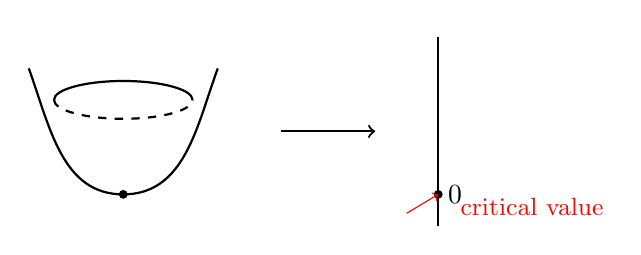
\begin{tikzpicture}[scale=0.8]
            % Paraboloid sketch
            \draw[thick] (-1.5,2.5) to[out=-70,in=180] (0,0.5) to[out=0,in=250] (1.5,2.5);
            \draw[thick,dashed] (-1.1,2) arc(180:360:1.1 and 0.3);
            \draw[thick] (-1.1,2) arc(180:0:1.1 and 0.3);
            \fill (0,0.5) circle (2pt);
            % Arrow
            \draw[->,thick] (2.5,1.5) -- (4,1.5);
            % R line
            \draw[thick] (5,0) -- (5,3);
            \node[right] at (5,3) {$\R$};
            \fill (5,0.5) circle (2pt) node[right] {$0$};
            \node[right,red] at (5.2,0.3) {\small critical value};
            \draw[<-,red] (5,0.5) -- (4.5,0.2);
        \end{tikzpicture}
        \end{center}

        \item $T^2 \to \R$ (height function on the torus). There are critical values at the top, bottom, and the two saddle points.

        \begin{center}
        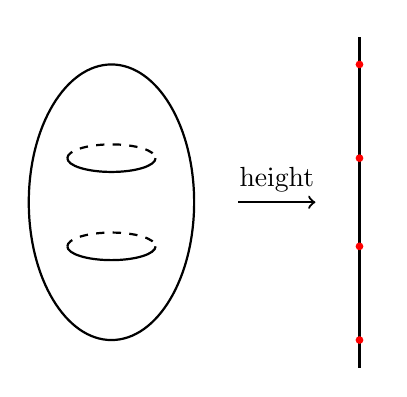
\begin{tikzpicture}[scale=0.7]
            % Torus outline (side view)
            \draw[thick] (0,0) ellipse (1.5 and 2.5);
            \draw[thick] (-0.8,0.8) arc(180:360:0.8 and 0.25);
            \draw[thick,dashed] (-0.8,0.8) arc(180:0:0.8 and 0.25);
            \draw[thick] (-0.8,-0.8) arc(180:360:0.8 and 0.25);
            \draw[thick,dashed] (-0.8,-0.8) arc(180:0:0.8 and 0.25);
            % Arrow
            \draw[->,thick] (2.3,0) -- (3.7,0) node[midway,above] {height};
            % R line
            \draw[thick] (4.5,-3) -- (4.5,3);
            \node[right] at (4.5,3) {$\R$};
            % Critical values
            \foreach \y/\lab in {2.5/top, 0.8/saddle, -0.8/saddle, -2.5/bottom} {
                \fill[red] (4.5,\y) circle (2pt);
            }
        \end{tikzpicture}
        \end{center}
    \end{enumerate}
\end{example}

\subsection{Application: Fundamental Theorem of Algebra}

As an application of these notions, let's prove the \emph{fundamental theorem of algebra}: every non-constant complex polynomial $P(z)$ must have a zero.

First, observe that if $M$ is compact, $q \in N$ is a regular value, and $\dim M = \dim N$, then $f^{-1}(q)$ is a finite set. Moreover, $\# f^{-1}(q)$ is a locally constant function of $q$ (as $q$ ranges only through regular values). (If $p_1, \ldots, p_k$ are points of $f^{-1}(q)$, then we can choose pairwise disjoint neighborhoods $U_1, \ldots, U_k$ mapping diffeomorphically onto $V_1, \ldots, V_k$. We may then take $V = V_1 \cap \cdots \cap V_k - f(M - U_1 - \cdots - U_k)$.)

\begin{proof}[Proof of the fundamental theorem of algebra]
    Consider the unit sphere $S^2 \subset \R^3$ and the stereographic projection
    \[
        h_+ \colon S^2 \setminus \{(0,0,1)\} \to \R^2 \times 0 \subset \R^3.
    \]
    \begin{center}
    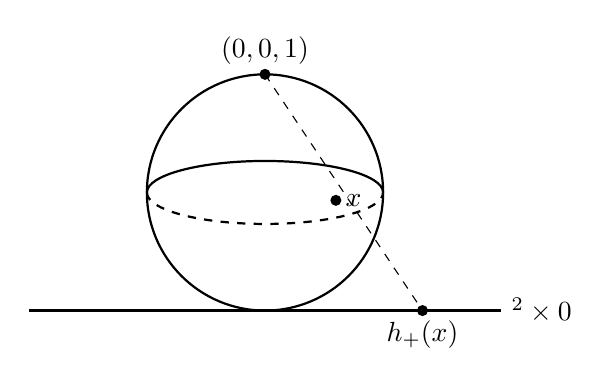
\begin{tikzpicture}[scale=1.0]
        % Sphere
        \draw[thick] (0,0) circle (1.5);
        \draw[thick,dashed] (-1.5,0) arc(180:360:1.5 and 0.4);
        \draw[thick] (-1.5,0) arc(180:0:1.5 and 0.4);
        % North pole
        \fill (0,1.5) circle (2pt) node[above] {$(0,0,1)$};
        % Plane
        \draw[thick] (-3,-1.5) -- (3,-1.5) node[right] {$\R^2 \times 0$};
        % Projection line
        \draw[dashed] (0,1.5) -- (2,-1.5);
        \fill (0.9,-0.1) circle (2pt) node[right] {$x$};
        \fill (2,-1.5) circle (2pt) node[below] {$h_+(x)$};
    \end{tikzpicture}
    \end{center}

    We identify $\R^2 \times 0$ with $\mathbb{C}$. Say $P(z) = a_0 z^n + a_1 z^{n-1} + \cdots + a_n$ with $a_0 \neq 0$.

    The polynomial map $P \colon \mathbb{C} \to \mathbb{C}$ corresponds to the map
    \begin{align*}
        f \colon S^2 &\to S^2 \\
        x &\mapsto h_+^{-1} \circ P \circ h_+(x) \quad \text{for } x \neq (0,0,1), \\
        (0,0,1) &\mapsto (0,0,1).
    \end{align*}

    The resulting map is smooth, even in a neighborhood of $(0,0,1)$. (Let $h_-$ be the stereographic projection from the south pole $(0,0,-1)$. Then $h_+ h_-^{-1}(z) = \frac{z}{|z|^2} = \frac{1}{\bar{z}}$, and $h_- \circ f \circ h_-^{-1}(z) = \frac{z^n}{\bar{a}_0 + \bar{a}_1 z + \cdots + \bar{a}_n z^n}$ is smooth at $0$.)

    Moreover, $f$ has only finitely many critical points, since $P'(z)$ is not identically zero. Hence, the set of regular values of $f$ is connected, and thus $\# f^{-1}(q)$ must be constant on this set. Since $\# f^{-1}(q)$ can't be zero everywhere, it is zero nowhere. Thus $f$ is surjective, and $P$ must have a zero.
\end{proof}


\chapter{Transversality, Homotopy, and Stability}
% lecture05.tex — Transversality, Homotopy, and Stability

\section{Transversality}

\begin{definition}{Transversality of Submanifolds}{transversal-submanifolds}
    We say two smooth submanifolds $M, M' \subset N$ are \emph{transversal} at $p \in M \cap M'$ if $T_p M + T_p M' = T_p N$. If they are transversal at every point $p \in M \cap M'$, we simply say they are \emph{transversal}, and write $M \pitchfork M'$.
\end{definition}

\begin{definition}{Transversality of a Map}{transversal-map}
    More generally, we say a smooth map $f \colon M \to N$ is \emph{transversal} to a submanifold $M' \subset N$ (abbreviated $f \pitchfork M'$) if
    \[
        \im(df_p) + T_q M' = T_q N \quad \text{for every } p \in f^{-1}(M'),
    \]
    where $q = f(p)$.
\end{definition}

\begin{center}
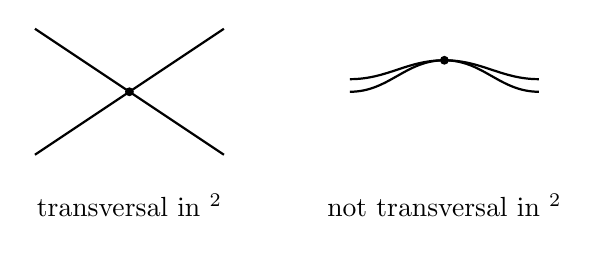
\begin{tikzpicture}[scale=0.8]
    % Transversal
    \draw[thick] (-1.5,-1) -- (1.5,1);
    \draw[thick] (-1.5,1) -- (1.5,-1);
    \fill (0,0) circle (2pt);
    \node at (0,-1.8) {transversal in $\R^2$};
    % Not transversal
    \begin{scope}[xshift=5cm]
        \draw[thick] (-1.5,0) to[out=0,in=180] (0,0.5) to[out=0,in=180] (1.5,0);
        \draw[thick] (-1.5,0.2) to[out=0,in=180] (0,0.5) to[out=0,in=180] (1.5,0.2);
        \fill (0,0.5) circle (2pt);
        \node at (0,-1.8) {not transversal in $\R^2$};
    \end{scope}
\end{tikzpicture}
\end{center}

The following theorem generalizes the preimage theorem for regular values:

\begin{theorem}{Transversal Preimage Theorem}{transversal-preimage}
    If $f \colon M \to N$ is a smooth map transversal to a submanifold $P \subset N$, then the preimage $f^{-1}(P) \subset M$ is a submanifold of $M$, whose codimension (i.e.\ $\dim M - \dim f^{-1}(P)$) equals that of $P \subset N$ (i.e.\ $\dim N - \dim P$).
\end{theorem}

\begin{proof}
    We need to show that every point $p \in f^{-1}(P)$ has a neighborhood $U$ in $M$ such that $f^{-1}(P) \cap U$ is a manifold.

    Let $q = f(p)$. In a neighborhood of $q$, we may write $P$ as the zero set of a collection of independent functions $g_1, \ldots, g_\ell$, where $\ell = \codim P = \dim N - \dim P$.

    \begin{center}
    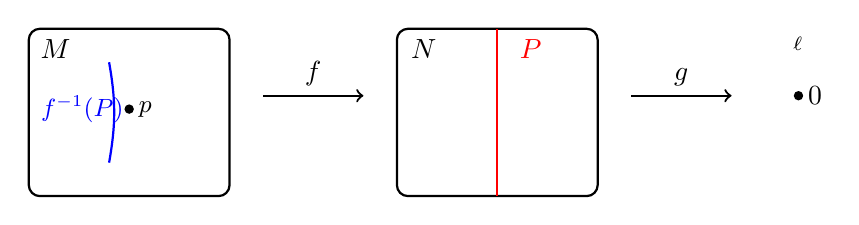
\begin{tikzpicture}[scale=0.85]
        % M with f^{-1}(P)
        \draw[thick,rounded corners] (-1.5,-1) rectangle (1.5,1.5);
        \node at (-1.1,1.2) {$M$};
        \draw[thick,blue] (-0.3,-0.5) to[out=80,in=280] (-0.3,1);
        \node[blue] at (-0.7,0.3) {\small $f^{-1}(P)$};
        \fill (0,0.3) circle (2pt) node[right] {\small $p$};
        % Arrow f
        \draw[->,thick] (2,0.5) -- (3.5,0.5) node[midway,above] {$f$};
        % N with P
        \draw[thick,rounded corners] (4,-1) rectangle (7,1.5);
        \node at (4.4,1.2) {$N$};
        \draw[thick,red] (5.5,-1) -- (5.5,1.5);
        \node[red] at (6,1.2) {$P$};
        % Arrow g
        \draw[->,thick] (7.5,0.5) -- (9,0.5) node[midway,above] {$g$};
        % R^l
        \fill (10,0.5) circle (2pt) node[right] {$0$};
        \node at (10,1.2) {$\R^\ell$};
    \end{tikzpicture}
    \end{center}

    Then, near $p$, $f^{-1}(P)$ is the zero set of $(g_1 \circ f, \ldots, g_\ell \circ f) = g \circ f$, so it's enough to show that $0$ is a regular value of $g \circ f$.

    Since $d(g \circ f)_p = dg_q \circ df_p$ and $dg_q \colon T_q N \to \R^\ell$ is surjective with $\ker dg_q = T_q P \subset T_q N$, $0$ is a regular value of $g \circ f$ if and only if $\im(df_p) + T_q P = T_q N$, which is exactly our transversality assumption.
\end{proof}

\begin{corollary}{Intersection of Transversal Submanifolds}{transversal-intersection}
    If $M, M' \subset N$ are two transversal submanifolds, then $M \cap M'$ is also a submanifold, with
    \[
        \codim(M \cap M') = \codim M + \codim M'.
    \]
\end{corollary}

\begin{remark}{Additivity of Codimension}{codim-additivity}
    Additivity of codimension is very natural. Think: cutting out a submanifold locally using $k = \codim M$ and $\ell = \codim M'$ independent functions.
\end{remark}

\section{Homotopy and Stability}

\begin{definition}{Homotopy}{homotopy}
    We say two smooth maps $f_0, f_1 \colon M \to N$ are \emph{homotopic}, abbreviated $f_0 \sim f_1$, if there exists a smooth map $F \colon M \times I \to N$ such that $F(x,0) = f_0(x)$ and $F(x,1) = f_1(x)$. We call such $F$ a \emph{homotopy} between $f_0$ and $f_1$.

    (Here $f_t(x) = F(x,t)$ is a smoothly evolving family of maps.)
\end{definition}

Homotopy is an equivalence relation on smooth maps from $M$ to $N$, and the equivalence class to which a map belongs is called its \emph{homotopy class}.

\begin{definition}{Stability}{stability}
    A property of smooth maps is called \emph{stable} if whenever $f_0 \colon M \to N$ possesses the property and $f_t \colon M \to N$ is a homotopy of $f_0$, then, for some $\varepsilon > 0$, each $f_t$ with $t < \varepsilon$ also possesses the property.
\end{definition}

\begin{theorem}{Stability Theorem}{stability-thm}
    The following classes of smooth maps of a \emph{compact} manifold $M$ into a manifold $N$ are stable classes:
    \begin{itemize}
        \item local diffeomorphisms,
        \item immersions,
        \item submersions,
        \item maps transversal to a given closed submanifold $P \subset N$,
        \item embeddings,
        \item diffeomorphisms.
    \end{itemize}
    (See Guillemin--Pollack pp.~36--37 for the proofs.)
\end{theorem}


\chapter{Sard's Theorem}
% lecture06.tex — Sard's Theorem

\section{Sard's Theorem}

\begin{theorem}{Sard's Theorem}{sard}
    Let $f \colon M \to N$ be a smooth map, and let
    \[
        C = \{x \in M \mid \rank\, df_x < \dim N\}
    \]
    be the set of critical points. Then, the set of critical values, $f(C)$, has measure zero in $N$.
\end{theorem}

\begin{proof}
    Thanks to second-countability of manifolds, it suffices to prove it for $f \colon U \to \R^p$, $U \overset{\text{open}}{\subset} \R^n$.

    We proceed by induction on $n$. Note, it is trivial for $n = 0$.

    Let
    \[
        C_1 = \{x \in U \mid df_x = 0\}
    \]
    and more generally
    \[
        C_k = \left\{x \in U \;\middle|\; \frac{\partial^j f}{\partial x_{s_1} \cdots \partial x_{s_j}}(x) = 0 \text{ for all } j \leq k \text{ and } 1 \leq s_1, \ldots, s_j \leq n\right\}.
    \]
    Thus we have a descending sequence of closed sets
    \[
        C \supset C_1 \supset C_2 \supset \cdots.
    \]

    We will prove the theorem in three steps:

    \textbf{Step 1:} $f(C - C_1)$ has measure zero.

    \textbf{Step 2:} $f(C_k - C_{k+1})$ has measure zero, for $k \geq 1$.

    \textbf{Step 3:} $f(C_k)$ has measure zero for $k$ sufficiently large.

    \begin{proof}[Proof of Step 1]
        We may assume $p \geq 2$, since $C = C_1$ when $p = 1$.

        We will use:
        \begin{theorem}{Fubini}{fubini}
            A measurable set $A \subset \R^p = \R \times \R^{p-1}$ must have measure zero if it intersects each hyperplane $(\text{const.}) \times \R^{p-1}$ in a set of $(p-1)$-dimensional measure zero.
        \end{theorem}

        For each $x \in C - C_1$, we will find an open neighborhood $V \subset \R^n$ so that $f(V \cap C)$ has measure zero.

        Since $x \notin C_1$, some partial derivative, say $\frac{\partial f_1}{\partial x_1}$, is nonzero at $x$. Consider the map $h \colon U \to \R^n$,
        \[
            x \mapsto (f_1(x), x_2, \ldots, x_n).
        \]
        Since $dh_x$ is nonsingular, it is a local diffeomorphism; it maps some neighborhood $V$ of $x$ diffeomorphically on to an open set $V' \subset \R^n$.

        \begin{center}
        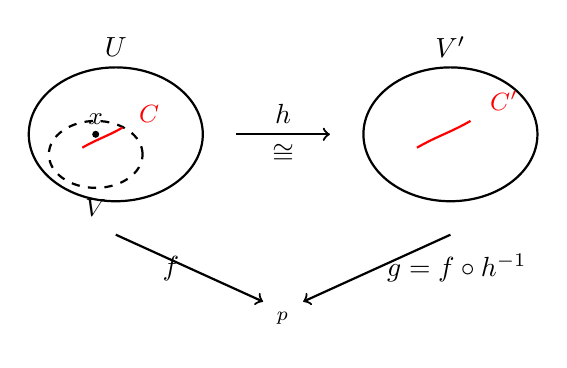
\begin{tikzpicture}[scale=0.85]
            % U with V, C
            \draw[thick] (0,0) ellipse (1.3 and 1);
            \node at (0,1.3) {$U$};
            \draw[thick,dashed] (-0.3,-0.3) ellipse (0.7 and 0.5);
            \node at (-0.3,-1.1) {\small $V$};
            \fill (-0.3,0) circle (1.5pt) node[above] {\small $x$};
            \draw[thick,red] (-0.5,-0.2) to[out=30,in=210] (0.1,0.1);
            \node[red] at (0.5,0.3) {\small $C$};
            % Arrow h
            \draw[->,thick] (1.8,0) -- (3.2,0) node[midway,above] {$h$} node[midway,below] {$\cong$};
            % V' with C'
            \draw[thick] (5,0) ellipse (1.3 and 1);
            \node at (5,1.3) {$V'$};
            \draw[thick,red] (4.5,-0.2) to[out=30,in=210] (5.3,0.2);
            \node[red] at (5.8,0.5) {\small $C'$};
            % Arrow f, g
            \draw[->,thick] (0,-1.5) -- (2.2,-2.5) node[midway,left] {$f$};
            \draw[->,thick] (5,-1.5) -- (2.8,-2.5) node[midway,right] {$g = f \circ h^{-1}$};
            \node at (2.5,-2.8) {$\R^p$};
        \end{tikzpicture}
        \end{center}

        Set $g := f \circ h^{-1}$. Then the set $C'$ of critical points of $g$ is $h(V \cap C)$, and the set $g(C')$ of critical values of $g$ is $f(V \cap C)$.

        Note, $g$ carries hyperplanes into hyperplanes; let
        \[
            g^t \colon (t \times \R^{n-1}) \cap V' \to t \times \R^{p-1}
        \]
        denote the restriction of $g$. Moreover, since
        \[
            \left(\frac{\partial g_i}{\partial x_j}\right) = \begin{pmatrix} 1 & 0 \\ * & \frac{\partial g^t_i}{\partial x_j} \end{pmatrix},
        \]
        a point of $t \times \R^{n-1}$ is critical for $g^t$ iff it is critical for $g$.

        By induction hypothesis, the set of critical values of $g^t$ has measure zero in $t \times \R^{p-1}$. Hence, by Fubini's theorem, the set
        \[
            g(C') = f(V \cap C)
        \]
        has measure zero, which completes Step 1.
    \end{proof}

    \begin{proof}[Proof of Step 2]
        (Similar to Step 1.)

        For each $x \in C_k - C_{k+1}$, some $(k+1)$-st derivative is nonzero, so let's say $w(x) = \frac{\partial^k f_r}{\partial x_{s_1} \cdots \partial x_{s_k}}$ vanishes at $x$ but $\frac{\partial w}{\partial x_1}$ does not.

        Then the map $h \colon U \to \R^n$, $x \mapsto (w(x), x_2, \ldots, x_n)$, carries some neighborhood $V$ diffeomorphically onto an open set $V' \subset \R^n$.

        Note, $h$ carries $C_k \cap V$ into the hyperplane $0 \times \R^{n-1}$. Hence, we can consider $g := f \circ h^{-1} \colon V' \to \R^p$ and its restriction $\bar{g} \colon (0 \times \R^{n-1}) \cap V' \to \R^p$.

        By induction, the set of critical values of $\bar{g}$ has measure $0$ in $\R^p$, and in particular, $\bar{g} \circ h(C_k \cap V) = f(C_k \cap V)$ has measure zero.
    \end{proof}

    \begin{proof}[Proof of Step 3]
        Let $I^n \subset U$ be a cube with edge $\delta$. We will prove that if $k$ is sufficiently large, $f(C_k \cap I^n)$ has measure zero. (The constant depends only on $f$ and $I^n$.)

        By Taylor's theorem, $f(x + h) = f(x) + R(x,h)$ where $\|R(x,h)\| \leq c\|h\|^{k+1}$ for $x \in C_k \cap I^n$, $x + h \in I^n$.

        Now, subdivide $I^n$ into $r^n$ cubes of edge $\frac{\delta}{r}$.

        Then, for each cube $I'$ in the subdivision containing a point $x \in C_k$, any other point of $I'$ can be written as $x + h$ with $\|h\| \leq \sqrt{n}\,\frac{\delta}{r}$, so
        \[
            \operatorname{Volume}(f(C_k \cap I')) \leq \left(2c\left(\sqrt{n}\,\frac{\delta}{r}\right)^{k+1}\right)^p.
        \]
        Therefore,
        \[
            \operatorname{Volume}(f(C_k \cap I^n)) \leq r^n \cdot \left(2c\left(\sqrt{n}\,\frac{\delta}{r}\right)^{k+1}\right)^p = c' \cdot r^{n - (k+1)p}
        \]
        which holds for any $r \in \Z_{>0}$, so we can send $r \to \infty$. And hence if $k + 1 > \frac{n}{p}$, $f(C_k \cap I^n)$ must have measure zero.

        This completes the proof of Sard's theorem.
    \end{proof}
\end{proof}


\chapter{Morse Functions}
% lecture07.tex — Morse Functions

\section{Morse Functions}

Consider a smooth function $f \colon M \to \R$. If $x \in M$ is a regular point of $f$ (i.e.\ if $df_x \neq 0$), we know that we can choose a local coordinate around $x$ so that $f$ is simply the first coordinate function.

What can we say at critical points?

Recall from calculus that a critical point $x$ of $f \colon \R^k \to \R$ is called \emph{nondegenerate} if the \emph{Hessian matrix} $H = \left(\frac{\partial^2 f}{\partial x_i \partial x_j}\right)$ is nonsingular at $x$.

\begin{center}
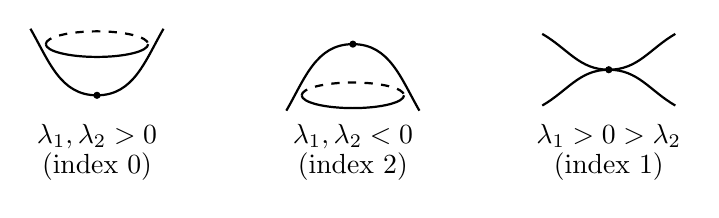
\begin{tikzpicture}[scale=0.65]
    % Index 0: bowl up
    \draw[thick] (-1.3,1.8) to[out=-60,in=180] (0,0.5) to[out=0,in=240] (1.3,1.8);
    \draw[thick] (-1,1.5) arc(180:360:1 and 0.25);
    \draw[thick,dashed] (-1,1.5) arc(180:0:1 and 0.25);
    \fill (0,0.5) circle (2pt);
    \node at (0,-0.3) {$\lambda_1, \lambda_2 > 0$};
    \node at (0,-0.9) {(index $0$)};
    % Index 2: bowl down
    \begin{scope}[xshift=5cm]
        \draw[thick] (-1.3,0.2) to[out=60,in=180] (0,1.5) to[out=0,in=120] (1.3,0.2);
        \draw[thick] (-1,0.5) arc(180:360:1 and 0.25);
        \draw[thick,dashed] (-1,0.5) arc(180:0:1 and 0.25);
        \fill (0,1.5) circle (2pt);
        \node at (0,-0.3) {$\lambda_1, \lambda_2 < 0$};
        \node at (0,-0.9) {(index $2$)};
    \end{scope}
    % Index 1: saddle
    \begin{scope}[xshift=10cm]
        \draw[thick] (-1.3,0.3) to[out=30,in=180] (0,1) to[out=0,in=150] (1.3,0.3);
        \draw[thick] (-1.3,1.7) to[out=-30,in=180] (0,1) to[out=0,in=210] (1.3,1.7);
        \fill (0,1) circle (2pt);
        \node at (0,-0.3) {$\lambda_1 > 0 > \lambda_2$};
        \node at (0,-0.9) {(index $1$)};
    \end{scope}
\end{tikzpicture}
\end{center}

\begin{proposition}{Nondegenerate Critical Points are Isolated}{nondeg-isolated}
    Nondegenerate critical points are isolated from the other critical points.
\end{proposition}

\begin{proof}
    Consider the map $\nabla f \colon \R^k \to \R^k$, $x \mapsto \left(\frac{\partial f}{\partial x_1}(x), \ldots, \frac{\partial f}{\partial x_k}(x)\right)$. Then $\nabla f(x) = 0$, since $x$ is a critical point. Nondegeneracy means $d(\nabla f)_x$ is a local diffeomorphism at $x$. Thus $f$ has no other critical point in a small neighborhood of $x$.
\end{proof}

\subsection{Nondegeneracy on Manifolds}

Nondegeneracy of critical points makes sense on manifolds, thanks to the following:

\begin{lemma}{Nondegeneracy is Independent of Coordinates}{nondeg-coords}
    Suppose $f \colon \R^k \to \R$ has a nondegenerate critical point at $0$ and $\psi$ is a diffeomorphism with $\psi(0) = 0$. Then $f \circ \psi$ also has a nondegenerate critical point at $0$.
\end{lemma}

\begin{proof}
    Let $f' = f \circ \psi$. Then
    \[
        \frac{\partial f'}{\partial x_i}(x) = \sum_\alpha \frac{\partial f}{\partial x_\alpha}(\psi(x)) \frac{\partial \psi_\alpha}{\partial x_i}(x),
    \]
    and
    \[
        \frac{\partial^2 f'}{\partial x_i \partial x_j}(0) = \sum_\alpha \sum_\beta \frac{\partial^2 f}{\partial x_\alpha \partial x_\beta}(0) \frac{\partial \psi_\alpha}{\partial x_i}(0) \frac{\partial \psi_\beta}{\partial x_j}(0) + \sum_\alpha \frac{\partial f}{\partial x_\alpha}(0) \frac{\partial^2 \psi_\alpha}{\partial x_i \partial x_j}(0).
    \]
    The last sum vanishes since $0$ is a critical point. That is, the new Hessian is $H' = (d\psi_0)^t H (d\psi_0)$. Since $H$ and $d\psi_0$ are nonsingular, so is $H'$.
\end{proof}

\begin{definition}{Morse Function}{morse-function}
    A function $f \colon M \to \R$ whose critical points are all nondegenerate is called a \emph{Morse function}.
\end{definition}

Morse functions are extremely important! They tell us a great deal about the topology of $M$, and much of modern topology is based on this idea. It'll take another whole course to talk about Morse theory, but let me just mention:

\emph{Morse lemma}: If $a \in M$ is a nondegenerate critical point of $f$, then there is a local coordinate system $(x_1, \ldots, x_m)$ around $a$ such that
\[
    f = f(a) + \sum h_{ij} x_i x_j \quad \text{near } a,
\]
i.e.\ $f$ is locally a quadratic polynomial.

\subsection{Abundance of Morse Functions}

As an application of Sard's theorem, let's show that the vast majority of functions are Morse functions.

\begin{theorem}{Generic Functions are Morse}{generic-morse}
    Let $f \colon M \to \R$ be a function, and suppose our manifold $M$ sits inside $\R^N$. For each $a = (a_1, \ldots, a_N) \in \R^N$, define
    \[
        f_a := f + a_1 x_1 + \cdots + a_N x_N,
    \]
    where $x_1, \ldots, x_N$ are the usual coordinate functions on $\R^N$. Then, for almost every $a \in \R^N$, $f_a$ is a Morse function.
\end{theorem}

\begin{proof}
    Let's first prove the result in $\R^k$:

    \begin{lemma}{Local Morse Genericity}{local-morse}
        Let $f \colon U \subset \R^k \to \R$ be a smooth function. Then, for almost all $a = (a_1, \ldots, a_k) \in \R^k$,
        \[
            f_a := f + a_1 x_1 + \cdots + a_k x_k
        \]
        is a Morse function on $U$.
    \end{lemma}

    \begin{proof}
        Note that $(df_a)_p = \left(\frac{\partial f_a}{\partial x_1}(p), \ldots, \frac{\partial f_a}{\partial x_k}(p)\right) = \nabla f(p) + a$, so $p$ is a critical point of $f_a$ iff $\nabla f(p) = -a$. Moreover, it's nondegenerate iff $d(\nabla f)_p$ is nonsingular, i.e.\ if $p$ is a regular point of $\nabla f$.

        Thanks to Sard, $-a$ is a regular value of $\nabla f$ for almost all $a \in \R^k$.
    \end{proof}

    Now let's turn this into a global result. Suppose $p \in M$ and $x_1, \ldots, x_N$ are the standard coordinate functions on $\R^N$. Then, some $m$ of these coordinate functions, $x_{i_1}, \ldots, x_{i_m}$, constitute a coordinate system in a neighborhood of $p$.

    Hence, we can cover $M$ with countably many such open subsets $U_\alpha$, and it suffices to show that $f_a$ is Morse on $U_\alpha$ for almost every $a \in \R^N$.

    For convenience, assume that $(x_1, \ldots, x_m)$ is a coordinate system on $U_\alpha$. Let $S_\alpha = \{a \in \R^N \mid f_a \text{ is not Morse on } U_\alpha\}$.

    Then, by the lemma, $S_\alpha \cap (\R^m \times \{c\})$ has measure zero in $\R^m$, for any $c = (c_{m+1}, \ldots, c_N)$. By Fubini, it follows that $S_\alpha$ has measure zero.
\end{proof}


\chapter{Whitney Embedding Theorem}
% lecture08.tex — Whitney Embedding Theorem

\section{Whitney Embedding Theorem}

So far, our $m$-manifold $M$ has been embedded in $\R^k$ where $k$ may be enormous. Can we embed it in a smaller Euclidean space?

\begin{theorem}{Strong Whitney Embedding Theorem}{strong-whitney}
    Any smooth $m$-manifold (with $m > 0$) can be embedded in $\R^{2m}$.
\end{theorem}

In this lecture, we'll only prove a weaker version where we embed it in $\R^{2m+1}$; going further down to $\R^{2m}$ requires a method known as the ``Whitney trick.''

Intuitively, it's clear why it should be possible to embed $M^m$ into $\R^{2m+1}$: since $m + m < 2m + 1$, there's enough room to wiggle things around.

\begin{center}
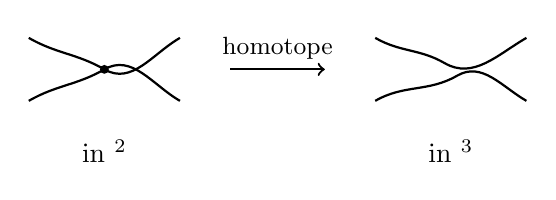
\begin{tikzpicture}[scale=0.8]
    % Self-intersecting in R^2
    \draw[thick] (-1.2,0.5) to[out=-30,in=150] (0,0) to[out=-30,in=210] (1.2,0.5);
    \draw[thick] (-1.2,-0.5) to[out=30,in=210] (0,0) to[out=30,in=150] (1.2,-0.5);
    \fill (0,0) circle (2pt);
    \node at (0,-1.3) {in $\R^2$};
    % Arrow
    \draw[->,thick] (2,0) -- (3.5,0) node[midway,above] {\small homotope};
    % Untangled in R^3
    \begin{scope}[xshift=5.5cm]
        \draw[thick] (-1.2,0.5) to[out=-30,in=150] (-0.1,0.1) to[out=-30,in=210] (1.2,0.5);
        \draw[thick] (-1.2,-0.5) to[out=30,in=210] (0.1,-0.1) to[out=30,in=150] (1.2,-0.5);
        \node at (0,-1.3) {in $\R^3$};
    \end{scope}
\end{tikzpicture}
\end{center}

\begin{remark}{}{whitney-optimal}
    Whitney's result is the best possible linear bound. In fact, when $m$ is a power of $2$, there's no embedding $\R\mathbb{P}^m \hookrightarrow \R^{2m-1}$.
\end{remark}

Now, let's prove:

\begin{theorem}{Injective Immersion in $\R^{2m+1}$}{injective-immersion}
    Every $m$-manifold admits an injective immersion in $\R^{2m+1}$.
\end{theorem}

\begin{proof}
    If $M^m \subset \R^k$, we will produce a linear projection $\R^k \to \R^{2m+1}$ that restricts to an injective immersion of $M$. Proceeding inductively, it suffices to show that: if $f \colon M \to \R^\ell$ is an injective immersion with $\ell > 2m + 1$, then there exists a unit vector $a \in \R^\ell$ such that the composition of $f$ with the projection map $\pi_a \colon \R^\ell \to H_a := \{b \in \R^\ell \mid b \perp a\}$ is still an injective immersion.

    Define maps
    \begin{align*}
        h \colon M \times M \times \R &\to \R^\ell, & (x, y, t) &\mapsto t(f(x) - f(y)), \\
        g \colon TM &\to \R^\ell, & (x, v) &\mapsto df_x(v).
    \end{align*}
    Since $\ell > 2m + 1$, by Sard, there exists a point $a \in \R^\ell \setminus \{0\}$ belonging to neither image.

    Then $\pi_a \circ f \colon M \to H_a$ is injective, since $\pi_a \circ f(x) = \pi_a \circ f(y) = ta$ implies either $t = 0$ (which means $x = y$ by injectivity of $f$) or $h(x, y, 1/t) = a$ (contradiction to our choice of $a$).

    Moreover, $\pi_a \circ f$ is an immersion, since $d(\pi_a \circ f)_x(v) = 0$ implies $\pi_a \circ df_x(v) = 0$, so $df_x(v) = ta$ for some $t \neq 0$ (by immersivity of $f$), which gives $g(x, v/t) = a$, a contradiction.
\end{proof}

For compact manifolds, injective immersions are the same as embeddings, so we have just proved the (weaker version of) embedding theorem in the compact case.

For non-compact manifolds, we need to modify the immersion to make it proper, which is a topological, not a differential problem. The fundamental technique for such generalization is the \emph{partition of unity}.

\begin{definition}{Partition of Unity}{partition-unity}
    Let $M$ be a smooth manifold. A \emph{partition of unity} $\{\rho_i\}_{i \in I}$ is a set of smooth functions $\rho_i \colon M \to \R$ such that
    \begin{enumerate}[label=(\alph*)]
        \item $\rho_i \geq 0$,
        \item each $x \in M$ has a neighborhood on which all but finitely many $\rho_i$ are identically zero,
        \item $\sum_{i \in I} \rho_i(x) = 1$ for all $x \in M$.
    \end{enumerate}

    If $\{U_\alpha\}_{\alpha \in A}$ is an open cover of $M$, then $\{\rho_i\}_{i \in I}$ is \emph{subordinate} to $\{U_\alpha\}_{\alpha \in A}$ if each $\operatorname{supp} \rho_i = \overline{\rho_i^{-1}(\R \setminus \{0\})}$ is contained in some $U_\alpha$.
\end{definition}

\begin{theorem}{Existence of Partitions of Unity}{partition-unity-existence}
    Every open cover $\{U_\alpha\}_{\alpha \in A}$ admits a countable partition of unity $\{\rho_i\}_{i \in I}$ subordinate to it.
\end{theorem}

(For now, let's take this theorem for granted.)

\begin{corollary}{Existence of Proper Functions}{proper-function}
    On any manifold $M$, there exists a proper function $f \colon M \to \R$.
\end{corollary}

\begin{proof}
    Let $\{U_\alpha\}_{\alpha \in A}$ be the set of open subsets of $M$ with compact closure. Choose a partition of unity $\{\rho_i\}_{i \in \Z_{>0}}$ subordinate to it. Define $f = \sum_{i=1}^{\infty} i\,\rho_i$. Then $f^{-1}([-j, j]) \subset \bigcup_{i=1}^{j} \operatorname{supp} \rho_i$, so $f$ is proper.
\end{proof}

Now we're ready to prove the:

\begin{theorem}{Whitney Embedding Theorem (Weak)}{whitney-weak}
    Every $m$-manifold embeds in $\R^{2m+1}$.
\end{theorem}

\begin{proof}
    Begin with an injective immersion $M \to \R^{2m+1}$. Composing with a diffeomorphism of $\R^{2m+1}$ into its unit ball, $z \mapsto \frac{z}{1 + |z|^2}$, we obtain an injective immersion $f \colon M \to \R^{2m+1}$ with $|f(x)| < 1$ for all $x \in M$.

    Let $g \colon M \to \R$ be a proper function, and define a new injective immersion
    \[
        F \colon M \to \R^{2m+2}, \qquad x \mapsto (f(x), g(x)).
    \]

    Recall that $\pi_a \circ F \colon M \to H_a \cong \R^{2m+1}$ is an injective immersion for almost every $a \in S^{2m+1}$, so pick an $a$ that is neither of the sphere's two poles.

    We claim that $\pi_a \circ F$ is proper. In fact, we will show that, for any $c$, there exists $d$ such that $(\pi_a \circ F)^{-1}(\bar{B}_c) \subset g^{-1}(\bar{B}_d)$, which is compact since $g$ is proper.

    If the claim is false, there should be a sequence of points $\{x_i\}$ in $M$ for which $|\pi_a \circ F(x_i)| < c$ but $g(x_i) \to \infty$.

    By the definition of $\pi_a$,
    \[
        w_i := \frac{1}{g(x_i)}\bigl(F(x_i) - \pi_a \circ F(x_i)\bigr) \in \R^{2m+2}
    \]
    is a multiple of $a$. As $i \to \infty$,
    \[
        w_i = \frac{F(x_i)}{g(x_i)} - \frac{\pi_a \circ F(x_i)}{g(x_i)} = \left(\frac{f(x_i)}{g(x_i)}, 1\right) - \frac{\pi_a \circ F(x_i)}{g(x_i)} \to (0, \ldots, 0, 1).
    \]
    Since each $w_i$ is a multiple of $a$, so should be the limit. This contradicts our choice of $a$, and therefore $\pi_a \circ F$ is proper.
\end{proof}


\chapter{Manifolds with Boundary}
% lecture09.tex — Manifolds with Boundary

\section{Manifolds with Boundary}

Consider the closed \emph{half-space}
\[
    H^m := \{(x_1, \ldots, x_m) \in \R^m \mid x_m \geq 0\}.
\]
The boundary $\partial H^m$ is defined to be the hyperplane $\R^{m-1} \times 0 \subset \R^m$.

\begin{definition}{Manifold with Boundary}{manifold-boundary}
    A subset $M \subset \R^k$ is called a \emph{smooth $m$-manifold with boundary} if it is locally diffeomorphic to $H^m$.
\end{definition}

The \emph{boundary} $\partial M$ is the set of all points of $M$ which correspond to points of $\partial H^m$ under such a local parametrization. Its complement is called the \emph{interior} $\operatorname{Int}(M) = M - \partial M$.

\begin{center}
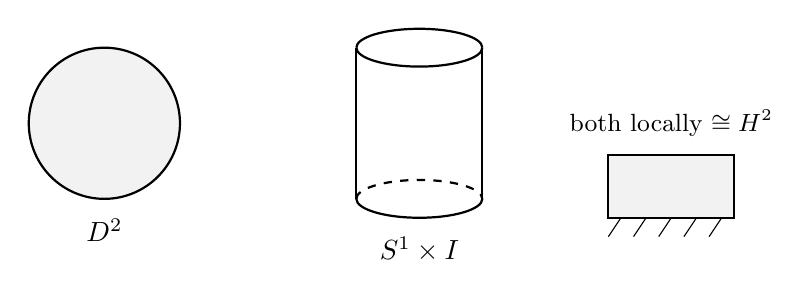
\begin{tikzpicture}[scale=0.8]
    % Disk D^2
    \draw[thick,fill=gray!10] (0,0) circle (1.2);
    \node at (0,-1.7) {$D^2$};
    % Cylinder S^1 x I
    \begin{scope}[xshift=5cm]
        \draw[thick] (-1,1.2) -- (-1,-1.2);
        \draw[thick] (1,1.2) -- (1,-1.2);
        \draw[thick] (-1,1.2) arc(180:360:1 and 0.3);
        \draw[thick] (-1,1.2) arc(180:0:1 and 0.3);
        \draw[thick] (-1,-1.2) arc(180:360:1 and 0.3);
        \draw[thick,dashed] (-1,-1.2) arc(180:0:1 and 0.3);
        \node at (0,-2) {$S^1 \times I$};
    \end{scope}
    % Label
    \node at (9,0) {\small both locally $\cong H^2$};
    % H^2
    \begin{scope}[xshift=9cm,yshift=-1.5cm]
        \draw[thick,fill=gray!10] (-1,0) rectangle (1,1);
        \draw[thick] (-1,0) -- (1,0);
        \foreach \x in {-0.8,-0.4,0,0.4,0.8} {
            \draw (\x,0) -- (\x-0.2,-0.3);
        }
    \end{scope}
\end{tikzpicture}
\end{center}

\begin{proposition}{Boundary is a Manifold}{boundary-manifold}
    If $M$ is a smooth $m$-manifold with boundary, $\partial M$ is a well-defined smooth $(m-1)$-manifold (without boundary).
\end{proposition}

\begin{proof}
    For any open neighborhood $U$ of $x \in \partial H^m$ in $H^m$, $U \cap \partial H^m$ is an open subset of $\partial H^m \cong \R^{m-1}$, so it suffices to show that any diffeomorphism between open subsets of $H^m$ sends boundary points to boundary points.

    Suppose $f \colon U \to V$ is such a diffeomorphism, and that it maps some $x \in \partial U$ to an interior point $y = f(x)$ of $V$. But then $f^{-1}$ must map an open neighborhood of $y$ in $\R^m$ (contained in $V$) onto an open neighborhood of $x$ in $\R^m$, which contradicts $x \in \partial U$.

    Therefore, $\partial M$ is a well-defined smooth $(m-1)$-manifold.
\end{proof}

The \emph{tangent space} $T_p M$ is defined just as before, so that it is a full $m$-dimensional vector space, even if $p \in \partial M$. In case $p \in \partial M$, there is a natural inclusion $T_p(\partial M) \hookrightarrow T_p M$ ($(m-1)$-dimensional into $m$-dimensional).

\begin{center}
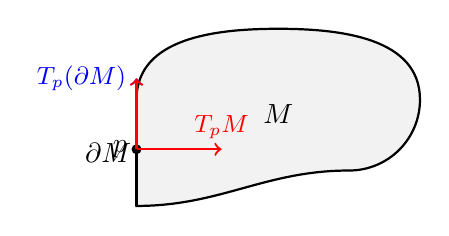
\begin{tikzpicture}[scale=0.9]
    % Manifold M with boundary
    \draw[thick,fill=gray!10] (0,0) to[out=0,in=180] (3,0.5) to[out=0,in=270] (4,1.5) to[out=90,in=0] (2,2.5) to[out=180,in=90] (0,1.5) -- cycle;
    \draw[very thick] (0,0) -- (0,1.5);
    \node at (2,1.3) {$M$};
    \node at (-0.4,0.75) {$\partial M$};
    % Point on boundary
    \fill (0,0.8) circle (2pt) node[left] {$p$};
    % T_p(∂M) — vertical
    \draw[->,thick,blue] (0,0.8) -- (0,1.8) node[left] {\small $T_p(\partial M)$};
    % T_pM — extends into M
    \draw[->,thick,red] (0,0.8) -- (1.2,0.8) node[above] {\small $T_p M$};
    \draw[->,thick,red] (0,0.8) -- (0,1.8);
\end{tikzpicture}
\end{center}

\subsection{Generating Examples}

Here's one method for generating examples:

\begin{lemma}{Preimage of a Regular Value}{preimage-boundary}
    Let $M$ be a manifold (without boundary) and let $g \colon M \to \R$ have $0$ as a regular value. Then $\{x \in M \mid g(x) \geq 0\}$ is a smooth manifold with boundary $g^{-1}(0)$.
\end{lemma}

\begin{proof}
    The set where $g > 0$ is open in $M$ and hence a submanifold of the same dimension. At points of $g^{-1}(0)$, $g$ is locally equivalent to the canonical submersion, and the lemma is obvious.
\end{proof}

\begin{example}{Unit Disk}{unit-disk}
    The unit disk $D^m = \{x \in \R^m \mid 1 - \sum_{i=1}^m x_i^2 \geq 0\}$ is a smooth manifold with boundary $\partial D^m = S^{m-1}$.
\end{example}

\subsection{Preimage Theorem with Boundary}

We also have a version of the preimage theorem:

\begin{theorem}{Preimage Theorem for Manifolds with Boundary}{preimage-boundary-thm}
    Let $f \colon M \to N$ be a smooth map from a manifold $M$ with boundary to a manifold $N$ (without boundary), and suppose that both $f \colon M \to N$ and $\partial f := f|_{\partial M} \colon \partial M \to N$ are transversal with respect to a submanifold $P \subset N$.

    Then, $f^{-1}(P) \subset M$ is a manifold with boundary $\partial f^{-1}(P) = f^{-1}(P) \cap \partial M$, and $\codim(f^{-1}(P) \subset M) = \codim(P \subset N)$.
\end{theorem}

\begin{proof}
    We only need to examine $f^{-1}(P)$ in a neighborhood of a point $x \in f^{-1}(P) \cap \partial M$, thanks to the earlier preimage theorem.

    As usual, in some neighborhood of $y = f(x) \in P$, there's a submersion $g$ to $\R^\ell$, $\ell = \codim(P \subset N)$, such that $P = g^{-1}(0)$ in this neighborhood.

    \begin{center}
    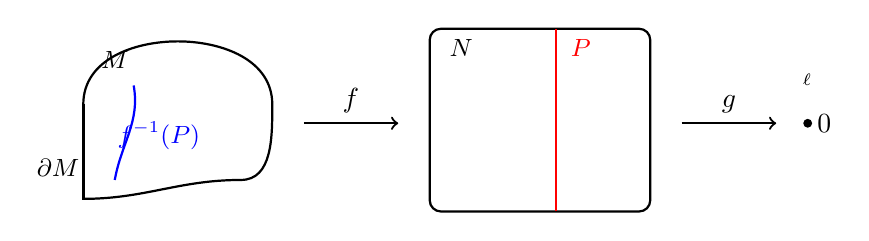
\begin{tikzpicture}[scale=0.8]
        % M with boundary, f^{-1}(P)
        \draw[thick] (0,0) to[out=0,in=180] (2.5,0.3) to[out=0,in=270] (3,1.5) to[out=90,in=0] (1.5,2.5) to[out=180,in=90] (0,1.5) -- cycle;
        \draw[very thick] (0,0) -- (0,1.5);
        \node at (0.5,2.2) {\small $M$};
        \node at (-0.4,0.5) {\small $\partial M$};
        \draw[thick,blue] (0.5,0.3) to[out=80,in=280] (0.8,1.8);
        \node[blue] at (1.2,1) {\small $f^{-1}(P)$};
        % Arrow
        \draw[->,thick] (3.5,1.2) -- (5,1.2) node[midway,above] {$f$};
        % N with P
        \draw[thick,rounded corners] (5.5,-0.2) rectangle (9,2.7);
        \node at (6,2.4) {\small $N$};
        \draw[thick,red] (7.5,-0.2) -- (7.5,2.7);
        \node[red] at (7.9,2.4) {\small $P$};
        % Arrow g
        \draw[->,thick] (9.5,1.2) -- (11,1.2) node[midway,above] {$g$};
        \fill (11.5,1.2) circle (2pt) node[right] {$0$};
        \node at (11.5,1.8) {\small $\R^\ell$};
    \end{tikzpicture}
    \end{center}

    Pre-composing with a local parametrization $\phi \colon U \subset H^m \to M$ around $x$, we obtain a map $h = g \circ f \circ \phi \colon U \subset H^m \to \R^\ell$ which is a submersion. By definition of smoothness, $h$ extends to a smooth map $\tilde{h}$ defined on a neighborhood $\tilde{U}$ of $u$ in $\R^m$, and the preimage $\tilde{h}^{-1}(0) \subset \tilde{U}$ is a manifold.

    Now, the transversality assumption on $\partial f$ implies that the last coordinate $x_m$ is regular on $\tilde{h}^{-1}(0)$ at $u$. Therefore, by the previous lemma, $\tilde{h}^{-1}(0) \cap \{x_m \geq 0\}$ is a manifold with boundary $\tilde{h}^{-1}(0) \cap \{x_m = 0\}$.
\end{proof}


\chapter{1-Manifolds and Some Consequences}
% lecture10.tex — 1-Manifolds and Some Consequences

\section{1-Manifolds and Some Consequences}

\begin{theorem}{Classification of 1-Manifolds}{classification-1-manifolds}
    Every compact, connected 1-manifold with boundary is diffeomorphic to $S^1$ or $I = [0,1]$.
\end{theorem}

(See the Appendix of Milnor or Guillemin--Pollack for the proof. The idea is to parametrize the 1-manifold by arc length, in a maximal way.)

\begin{corollary}{Boundary Has Even Cardinality}{boundary-even}
    The boundary of any compact 1-manifold with boundary consists of an even number of points.
\end{corollary}

As we will see, this seemingly trivial corollary has numerous nontrivial applications.

Later, in the next chapter, we will refine this statement by counting those boundary points with sign (orientation). Such signed count is always $0$, and this fact is at the heart of \emph{oriented intersection theory}.

\subsection{No Retraction Lemma}

Let $M$ be a compact manifold with boundary.

\begin{lemma}{No Retraction}{no-retraction}
    There's no smooth map $f \colon M \to \partial M$ that leaves $\partial M$ pointwise fixed. That is, there is no retraction of $M$ onto $\partial M$.
\end{lemma}

\begin{proof}
    Suppose there were such a map $f$. Let $y \in \partial M$ be a regular value for $f$ (which exists thanks to Sard). Since $y$ is certainly a regular value for the identity map $f|_{\partial M}$ as well, $f^{-1}(y)$ is a smooth 1-manifold, with boundary
    \[
        \partial f^{-1}(y) = f^{-1}(y) \cap \partial M = \{y\}.
    \]
    But $f^{-1}(y)$ is also compact, so that $\#|\partial f^{-1}(y)|$ must be even, a contradiction.
\end{proof}

\subsection{Brouwer Fixed Point Theorem}

\begin{theorem}{Smooth Brouwer Fixed Point Theorem}{smooth-brouwer}
    Any smooth map $g \colon D^n \to D^n$ has a fixed point.
\end{theorem}

\begin{proof}
    Suppose $g$ has no fixed point. Then we can construct a retraction $f \colon D^n \to S^{n-1}$ which is impossible from the lemma:
    \begin{center}
    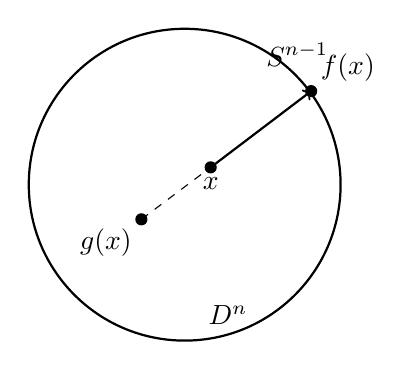
\begin{tikzpicture}[scale=1.1]
        % Disk
        \draw[thick] (0,0) circle (1.8);
        \node at (1.3,1.5) {$S^{n-1}$};
        \node at (0.5,-1.5) {$D^n$};
        % Points
        \fill (0.3,0.2) circle (2pt) node[below] {$x$};
        \fill (-0.5,-0.4) circle (2pt) node[below left] {$g(x)$};
        % Ray from g(x) through x to boundary
        \draw[dashed] (-0.5,-0.4) -- (0.3,0.2);
        \draw[->,thick] (0.3,0.2) -- (1.46,1.08);
        \fill (1.46,1.08) circle (2pt) node[above right] {$f(x)$};
    \end{tikzpicture}
    \end{center}
    \[
        f(x) = x + tu, \quad \text{where } u = \frac{x - g(x)}{\|x - g(x)\|} \text{ and } t = -x \cdot u + \sqrt{1 - x \cdot x + (x \cdot u)^2}.
    \]
    Note $t$ is strictly positive.
\end{proof}

Often, one can use an approximation theorem to pass to the continuous case, and this theorem is an example:

\begin{theorem}{Brouwer Fixed Point Theorem}{brouwer}
    Any continuous map $G \colon D^n \to D^n$ has a fixed point.
\end{theorem}

\begin{proof}
    Given $\varepsilon > 0$, thanks to the Weierstrass approximation theorem, there is a polynomial function $P_0 \colon \R^n \to \R^n$ with $\|P_0(x) - G(x)\| < \varepsilon$ for $x \in D^n$.

    However, $P_0$ may send points of $D^n$ into points outside of $D^n$, so to correct this we set $P(x) = \frac{P_0(x)}{1 + \varepsilon}$.

    Clearly, $P \colon D^n \to D^n$ and $\|P(x) - G(x)\| < \frac{2\varepsilon}{1+\varepsilon} < 2\varepsilon$ for $x \in D^n$.

    Suppose $G$ has no fixed points. Then the continuous function $\|G(x) - x\|$ must take on a minimum $\mu > 0$ on $D^n$. Choosing $P \colon D^n \to D^n$ as above, with $\|P(x) - G(x)\| < \mu$ for all $x \in D^n$, we have $P(x) \neq x$ for all $x \in D^n$.

    Since $P$ is smooth, this contradicts the Smooth Brouwer fixed point theorem.
\end{proof}

\subsection{The Hex Theorem}

The following is just for fun:

\begin{theorem}{Hex Theorem}{hex}
    There's no draw in the game of Hex. That is, if we color the vertices of a triangulation of $I^2$ in 2 colors, say red and blue, then either the red connects E--W or the blue connects N--S.
\end{theorem}

\begin{proof}
    \begin{center}
    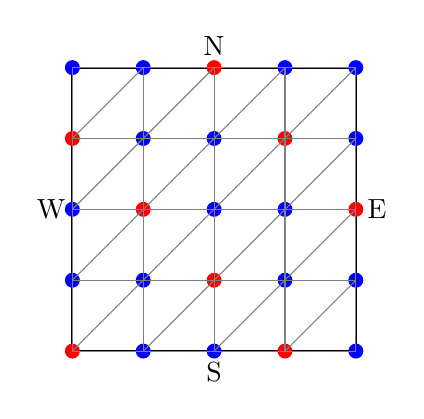
\begin{tikzpicture}[scale=0.9]
        % Square
        \draw[thick] (0,0) rectangle (4,4);
        \node at (2,4.3) {N};
        \node at (2,-0.3) {S};
        \node at (-0.3,2) {W};
        \node at (4.3,2) {E};
        % Grid of vertices
        \foreach \x in {0,1,2,3,4} {
            \foreach \y in {0,1,2,3,4} {
                \pgfmathparse{mod(\x+\y,3)==0 ? 1 : 0}
                \ifnum\pgfmathresult=1
                    \fill[red] (\x,\y) circle (3pt);
                \else
                    \fill[blue] (\x,\y) circle (3pt);
                \fi
            }
        }
        % Triangulation lines (some diagonals)
        \foreach \x in {0,1,2,3} {
            \foreach \y in {0,1,2,3} {
                \draw[gray,thin] (\x,\y) -- (\x+1,\y+1);
            }
        }
        % Horizontal and vertical grid
        \foreach \x in {0,1,2,3,4} {
            \draw[gray,thin] (\x,0) -- (\x,4);
        }
        \foreach \y in {0,1,2,3,4} {
            \draw[gray,thin] (0,\y) -- (4,\y);
        }
    \end{tikzpicture}
    \end{center}

    Suppose there is a coloring for which neither red nor blue connects the two opposite sides. Then, we can construct a continuous map $f \colon I^2 \to I^2$ without any fixed point, which contradicts the Brouwer fixed point theorem.

    We construct such $f$ as follows: For each vertex $v$ of the triangulation, set
    \[
        f(v) = \begin{cases}
            v + (\varepsilon, 0) & \text{if } v \text{ is colored in red and connected to W}, \\
            v - (\varepsilon, 0) & \text{if } v \text{ is colored in red and not connected to W}, \\
            v + (0, \varepsilon) & \text{if } v \text{ is colored in blue and connected to S}, \\
            v - (0, \varepsilon) & \text{if } v \text{ is colored in blue and not connected to S}.
        \end{cases}
    \]
    Extend linearly on each simplex. Then $f$ has no fixed points.
\end{proof}


\chapter{Transversality}
% lecture11.tex — Transversality

\section{Transversality}

Earlier, we saw that transversality is stable under small perturbations. Today, we'll use Sard's theorem to show that transversal maps are \emph{generic} in the sense that any smooth map can be deformed by an arbitrarily small amount into a transversal map.

(Think as a smooth family of maps $f_s \colon M \to N$, $s \in S$.)

\begin{theorem}{Transversality Theorem}{transversality-thm}
    Suppose $F \colon M \times S \to N$ is a smooth map of manifolds, where only $M$ has $\partial$, and let $P \subset N$ be a submanifold. If both $F$ and $F|_{\partial M \times S}$ are transversal to $P$, then for almost every $s \in S$, both $f_s$ and $f_s|_{\partial M}$ are transversal to $P$.
\end{theorem}

\begin{proof}
    The preimage $Q = F^{-1}(P) \subset M \times S$ is a submanifold with boundary $\partial Q = Q \cap (\partial M \times S)$. Let $\pi \colon Q \to S$ be the projection.

    We'll show that \textcircled{1} $f_s \pitchfork P$ whenever $s$ is a regular value for $\pi$, and \textcircled{2} $f_s|_{\partial M} \pitchfork P$ whenever $s$ is a regular value for $\pi|_{\partial Q}$. The theorem will then follow from Sard.

    Note that the second claim is a special instance of the first claim, for the map $F|_{\partial M \times S} \colon \partial M \times S \to N$ of boundaryless manifolds, so it suffices to show \textcircled{1}.

    In order to show $f_s \pitchfork P$, we need to show that, for any $x \in M$ with $f_s(x) = y \in P$, the composition $T_x M \xrightarrow{d(f_s)_x} T_y N \xrightarrow{p} T_y N / T_y P$ is surjective. (Here $d(f_s)_x(v) = dF_{(x,s)}(v, 0)$.)

    Since $F \pitchfork P$, we know that
    \[
        T_{(x,s)}(M \times S) = T_x M \times T_s S \xrightarrow{dF_{(x,s)}} T_y N \xrightarrow{p} T_y N / T_y P
    \]
    is surjective. Moreover, by the regularity assumption, $d\pi_{(x,s)} \colon T_{(x,s)} Q \to T_s S$ is surjective.

    Since $T_{(x,s)} Q \subset T_x M \times T_s S$ is in the kernel of $p \circ dF_{(x,s)}$, it follows that the restriction $p \circ dF_{(x,s)}|_{T_x M \times 0} = p \circ d(f_s)_x$ is surjective, as desired.
\end{proof}

\begin{corollary}{Transversal Maps are Generic (Euclidean Target)}{transversal-generic-euclidean}
    Transversal maps are generic when the target manifold $N$ is $\R^\ell$.
\end{corollary}

\begin{proof}
    If $f \colon M \to \R^\ell$ is any smooth map, take $S$ to be an open ball of $\R^\ell$, and define $F \colon M \times S \to \R^\ell$, $(x, s) \mapsto f(x) + s$.

    For any fixed $x$, this is obviously a submersion, so transversal to any submanifold $P \subset \R^\ell$.

    Thanks to the transversality theorem, $f_s(x) = f(x) + s$ is transversal to $P$, for almost every $s \in S$, where $s$ may be taken to be arbitrarily small.
\end{proof}

For an arbitrary target manifold $N \subset \R^\ell$, the proof of genericity of transversal maps is essentially the same; we just need to project the shifted map down to $N$.

\begin{lemma}{$\varepsilon$-Neighborhood Theorem}{epsilon-neighborhood}
    For any manifold $N \subset \R^\ell$, there is a smooth positive function $\varepsilon \colon N \to \R_{>0}$ such that each point $w \in N^\varepsilon := \{w \in \R^\ell \mid \|w - y\| < \varepsilon(y) \text{ for some } y \in N\}$ has a unique closest point $\pi(w)$ in $N$. Moreover, the map $\pi \colon N^\varepsilon \to N$ is a submersion.

    (See pp.~71--72 of Guillemin--Pollack for the proof.)
\end{lemma}

\begin{center}
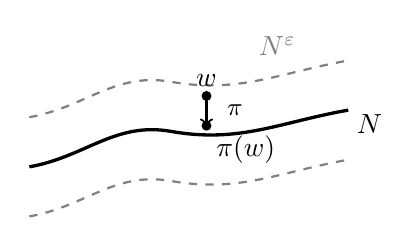
\begin{tikzpicture}[scale=0.9]
    % Manifold N (curve)
    \draw[very thick] (-2,-0.5) to[out=10,in=170] (0,0) to[out=-10,in=190] (2.5,0.3);
    \node at (2.8,0.1) {$N$};
    % Epsilon neighborhood (tube)
    \draw[thick,dashed,gray] (-2,-0.5+0.7) to[out=10,in=170] (0,0.7) to[out=-10,in=190] (2.5,1);
    \draw[thick,dashed,gray] (-2,-0.5-0.7) to[out=10,in=170] (0,-0.7) to[out=-10,in=190] (2.5,-0.4);
    \node[gray] at (1.5,1.2) {$N^\varepsilon$};
    % Point w and projection
    \fill (0.5,0.5) circle (2pt) node[above] {$w$};
    \draw[->,thick] (0.5,0.5) -- (0.5,0.08);
    \fill (0.5,0.08) circle (2pt) node[below right] {$\pi(w)$};
    \node at (0.9,0.3) {\small $\pi$};
\end{tikzpicture}
\end{center}

\begin{corollary}{Submersive Family}{submersive-family}
    Let $f \colon M \to N$ be a smooth map, where only $M$ has boundary. Then there is an open ball $S$ in some Euclidean space and a smooth map $F \colon M \times S \to N$ such that $F(x, 0) = f(x)$, and for any fixed $x \in M$, the map $S \to N$, $s \mapsto F(x, s)$, is a submersion. In particular, both $F$ and $F|_{\partial M \times S}$ are submersions.
\end{corollary}

\begin{proof}
    Let $S$ be the unit open ball in $\R^\ell \supset N$, and define
    \[
        F(x, s) = \pi\bigl(f(x) + \varepsilon(f(x)) s\bigr).
    \]
    Since $\pi \colon N^\varepsilon \to N$ restricts to the identity on $N$, $F(x, 0) = f(x)$. Since $s \mapsto f(x) + \varepsilon(f(x)) s$ and $\pi$ are compositions of two submersions, it is a submersion.
\end{proof}

\subsection{Transversality Homotopy and Extension Theorems}

\begin{theorem}{Transversality Homotopy Theorem}{transversality-homotopy}
    For any smooth map $f \colon M \to N$ and a submanifold $P \subset N$, where only $M$ has $\partial$, there exists a smooth map $g \colon M \to N$ homotopic to $f$ such that $g \pitchfork P$ and $g|_{\partial M} \pitchfork P$.
\end{theorem}

\begin{proof}
    For the family of maps $F$ in the corollary, the transversality theorem implies that $f_s \pitchfork P$ and $f_s|_{\partial M} \pitchfork P$ for almost all $s \in S$, but each $f_s$ is homotopic to $f$, with homotopy $M \times I \to N$, $(x, t) \mapsto F(x, ts)$.
\end{proof}

We'll actually need a slightly stronger form of this theorem:

\begin{theorem}{Extension Theorem (Relative Transversality Homotopy)}{extension-thm}
    In the setting as above, where $P$ is a closed submanifold, suppose $C \subset M$ is a closed subset such that $f \pitchfork P$ on $C$ and $f|_{\partial M} \pitchfork P$ on $C \cap \partial M$.

    Then there exists a smooth map $g \colon M \to N$ homotopic to $f$ such that $g \pitchfork P$, $g|_{\partial M} \pitchfork P$, and $g = f$ on a neighborhood of $C$.

    (See pp.~72--73 of Guillemin--Pollack for the proof. The idea is to modify $F \colon M \times S \to N$ where $\tau \colon M \to [0,1]$ is a smooth bump function that is $0$ on $C$ and $1$ outside of an open neighborhood, by setting $G \colon M \times S \to N$, $(x, s) \mapsto F(x, \tau(x) s)$.)
\end{theorem}

\begin{corollary}{Extension of Transversality}{extension-transversality}
    If $f \colon M \to N$ is a smooth map such that $f|_{\partial M} \colon \partial M \to N$ is transversal to $P \subset N$, then there exists a map $g \colon M \to N$ homotopic to $f$ rel $\partial$ (i.e.\ $g|_{\partial M} = f|_{\partial M}$) such that $g \pitchfork P$.
\end{corollary}


\chapter{Mod 2 Intersection Theory}
% lecture12.tex — Mod 2 Intersection Theory

\section{Mod 2 Intersection Theory}

Consider two closed submanifolds $M_1, M_2 \subset N$ of complementary dimension (i.e.\ $\dim M_1 + \dim M_2 = \dim N$), where at least one of $M_1$ or $M_2$ is compact.

When they intersect transversely, $M_1 \cap M_2$ must be a compact $0$-manifold (i.e.\ a finite set of points), so we can count the ``intersection number'' $\#(M_1 \cap M_2)$.

Even if their intersection is not transverse, we know we can homotope them to make it transverse.

\begin{center}
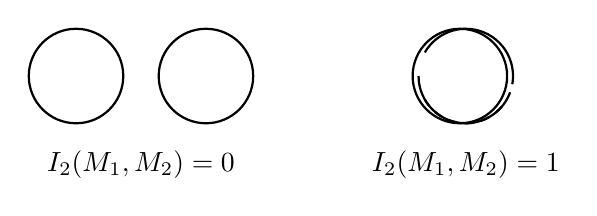
\begin{tikzpicture}[scale=0.75]
    % Unlinked circles
    \draw[thick] (0,0) circle (0.8);
    \draw[thick] (2.2,0) circle (0.8);
    \node at (1.1,-1.5) {$I_2(M_1, M_2) = 0$};
    % Linked circles
    \begin{scope}[xshift=6.5cm]
        \draw[thick] (0,0) circle (0.8);
        \draw[thick] (0.9,0) arc(0:150:0.8);
        \draw[thick,dashed] (0.9,0) arc(0:-150:0.8);
        \draw[thick] (-0.7,0) arc(180:330:0.8);
        \node at (0.1,-1.5) {$I_2(M_1, M_2) = 1$};
    \end{scope}
\end{tikzpicture}
\end{center}

Depending on the choice of homotopy, the number of intersections might change, but we'll show that the \emph{mod 2 intersection number} is well-defined.

\begin{definition}{Mod 2 Intersection Number}{mod2-intersection}
    Suppose $M_1$ is a compact manifold, $f \colon M_1 \to N$ is a smooth map, $M_2 \subset N$ is a closed submanifold with $\dim M_1 + \dim M_2 = \dim N$. Choose any map $g$ homotopic to $f$ and transversal to $M_2$. Define the \emph{mod 2 intersection number} of $f$ with $M_2$, $I_2(f, M_2)$, to be
    \[
        \# g^{-1}(M_2) \mod 2 \quad \in \Z/2\Z.
    \]
\end{definition}

\begin{theorem}{Mod 2 Intersection Number is Well-Defined}{mod2-well-defined}
    If $g_0, g_1 \colon M_1 \to N$ are homotopic and both transversal to $M_2 \subset N$, then $\# g_0^{-1}(M_2) = \# g_1^{-1}(M_2) \mod 2$.

    In particular, the mod 2 intersection number is well-defined and invariant under homotopy.
\end{theorem}

\begin{proof}
    Let $G \colon M_1 \times I \to N$ be a homotopy of $g_0$ and $g_1$. By the relative transversality homotopy theorem, we may assume $G \pitchfork M_2$. Then $G^{-1}(M_2)$ is a 1-dimensional submanifold of $M_1 \times I$ with boundary
    \[
        \partial G^{-1}(M_2) = G^{-1}(M_2) \cap \partial(M_1 \times I) = g_0^{-1}(M_2) \times \{0\} \cup g_1^{-1}(M_2) \times \{1\}.
    \]
    \begin{center}
    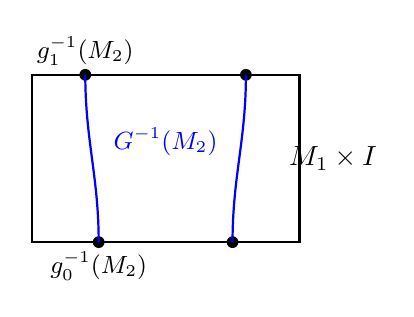
\begin{tikzpicture}[scale=0.85]
        % M_1 x I rectangle
        \draw[thick] (0,0) rectangle (4,2.5);
        \node at (4.5,1.25) {$M_1 \times I$};
        % Bottom: g_0^{-1}(M_2)
        \fill (1,0) circle (2.5pt) node[below] {\small $g_0^{-1}(M_2)$};
        \fill (3,0) circle (2.5pt);
        % Top: g_1^{-1}(M_2)
        \fill (0.8,2.5) circle (2.5pt) node[above] {\small $g_1^{-1}(M_2)$};
        \fill (3.2,2.5) circle (2.5pt);
        % Cobordism curves
        \draw[thick,blue] (1,0) to[out=90,in=270] (0.8,2.5);
        \draw[thick,blue] (3,0) to[out=90,in=270] (3.2,2.5);
        \node[blue] at (2,1.5) {\small $G^{-1}(M_2)$};
    \end{tikzpicture}
    \end{center}
    Since the boundary of any compact 1-manifold has an even number of points, $\# g_0^{-1}(M_2) + \# g_1^{-1}(M_2)$ is even.
\end{proof}

\begin{example}{Mod 2 Intersection Numbers}{mod2-examples}
    \begin{enumerate}
        \item Let $D \subset \R^3$ be a disk and $S^1 \subset \R^3$ a circle, with $\partial D$ unlinked from $S^1$. Then $I_2(D, S^1) = 0$, since $D$ may be chosen disjoint from $S^1$. (Dim check: $\dim D + \dim S^1 = 2 + 1 = 3 = \dim \R^3$.)
        \item Let $D \subset \R^3$ be a disk and $S^1 \subset \R^3$ a circle, with $\partial D$ linked with $S^1$. Then $I_2(D, S^1) = 1$, since every disk bounded by $\partial D$ must be punctured by $S^1$ an odd number of times.
        \item The core circle $M$ of a M\"obius band $N$: the mod 2 self-intersection number $I_2(M, M) = 1$.
    \end{enumerate}
\end{example}

% Examples are illustrated by the linked/unlinked diagrams above and the Mobius band diagram below

\subsection{Boundary Theorem}

\begin{theorem}{Boundary Theorem}{boundary-thm}
    Suppose that $M_1$ is the boundary of some compact manifold $W$ and $f \colon M_1 \to N$ is a smooth map. If $f$ can be extended to all of $W$, then $I_2(f, M_2) = 0$ for any closed submanifold $M_2 \subset N$ of complementary dimension.
\end{theorem}

\begin{proof}
    Let $F \colon W \to N$ extend $f$, which we may assume to be transversal to $M_2$, by the transversality homotopy theorem. Then $F^{-1}(M_2)$ is a compact 1-manifold with boundary $\partial F^{-1}(M_2) = f^{-1}(M_2)$, so $\# f^{-1}(M_2)$ must be even.
    \begin{center}
    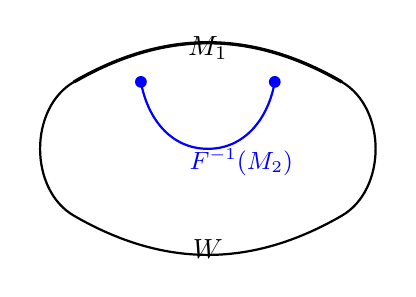
\begin{tikzpicture}[scale=0.85]
        % W (blob)
        \draw[thick] (0,0) to[out=30,in=150] (4,0) to[out=-30,in=30] (4,-2) to[out=210,in=330] (0,-2) to[out=150,in=210] cycle;
        \node at (2,-2.5) {$W$};
        % M_1 = boundary (top part)
        \draw[very thick] (0,0) to[out=30,in=150] (4,0);
        \node at (2,0.5) {$M_1$};
        % F^{-1}(M_2) curves with boundary on M_1
        \draw[thick,blue] (1,0) to[out=-80,in=180] (2,-1) to[out=0,in=260] (3,0);
        \fill[blue] (1,0) circle (2.5pt);
        \fill[blue] (3,0) circle (2.5pt);
        \node[blue] at (2.5,-1.2) {\small $F^{-1}(M_2)$};
    \end{tikzpicture}
    \end{center}
\end{proof}

\subsection{Mod 2 Degree}

\begin{definition}{Mod 2 Degree}{mod2-degree}
    If $f \colon M \to N$ is a smooth map of a compact manifold $M$ into a connected manifold $N$ of the same dimension, define the \emph{mod 2 degree} of $f$,
    \[
        \deg_{\Z/2}(f), \text{ to be } I_2(f, \{y\}), \text{ for any point } y \in N.
    \]
\end{definition}

\begin{theorem}{Mod 2 Degree is Well-Defined}{mod2-degree-well-defined}
    Mod 2 degree is well-defined.
\end{theorem}

\begin{proof}
    For any $y \in N$, we can homotope $f$ to make it transversal to $\{y\}$. From Lecture 4, we know $y \mapsto I_2(f, \{y\})$ is locally constant. Since $N$ is connected, it must be globally constant.
\end{proof}

Since $\deg_{\Z/2}$ is defined as an intersection number, we immediately obtain:

\begin{theorem}{}{mod2-degree-homotopy}
    The mod 2 degree is invariant under homotopy.
\end{theorem}

\begin{theorem}{}{mod2-degree-boundary}
    If $M = \partial W$ and $f \colon M \to N$ extends to all of $W$, then $\deg_{\Z/2}(f) = 0$.
\end{theorem}

\begin{example}{Mod 2 Degree Examples}{mod2-degree-examples}
    A constant map $c \colon M \to M$, $x \mapsto c$, has $\deg_{\Z/2}(c) = 0$.

    The identity map $\id \colon M \to M$, $x \mapsto x$, has $\deg_{\Z/2}(\id) = 1$.

    In particular, the identity map of a compact manifold (without boundary) is NOT homotopic to a constant map.

    (In case $M = \partial W$, this implies that $\id \colon M \to M$ cannot be extended to all of $W$, a result we saw in Lecture 10.)
\end{example}


\chapter{Winding Number and Borsuk--Ulam Theorem}
% lecture13.tex — Winding Number and Borsuk-Ulam Theorem

\section{Winding Numbers}

\begin{definition}{Winding Number}{winding-number}
    Let $M$ be a compact, connected $(n-1)$-manifold and $f \colon M \to \R^n$ a smooth map. If $z \in \R^n$ is not in the image of $f$, consider the map
    \[
        u \colon M \to S^{n-1}, \qquad x \mapsto \frac{f(x) - z}{|f(x) - z|}.
    \]
    Define the \emph{mod 2 winding number} of $f$ around $z$ to be the mod 2 degree of $u$, i.e.
    \[
        \operatorname{wind}_{\Z/2}(f, z) := \deg_{\Z/2}(u).
    \]
\end{definition}

\begin{center}
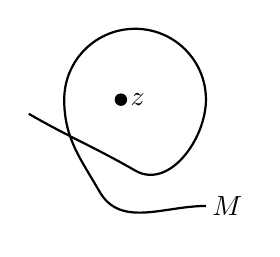
\begin{tikzpicture}[scale=0.9]
    % Curve M
    \draw[thick] (0,0.8) to[out=-30,in=150] (1.5,0) to[out=-30,in=270] (2.5,1) to[out=90,in=0] (1.5,2) to[out=180,in=90] (0.5,1) to[out=270,in=120] (1,-0.3) to[out=300,in=180] (2.5,-0.5);
    \node at (2.8,-0.5) {$M$};
    % Point z
    \fill (1.3,1) circle (2.5pt) node[right] {$z$};
\end{tikzpicture}
\end{center}

\begin{theorem}{Winding Number Formula}{winding-formula}
    Suppose $M = \partial D$ for some compact $n$-manifold $D$ with boundary, and let $F \colon D \to \R^n$ be a map extending $f$. If $z \in \R^n$ is a regular value of $F$ that's not in the image of $f$, then
    \[
        \operatorname{wind}_{\Z/2}(f, z) = \# F^{-1}(z) \mod 2.
    \]
\end{theorem}

\begin{proof}
    If $z$ is not in the image of $F$, then $u$ extends to $D$, so $\deg_{\Z/2}(u) = 0$ in that case.

    If $F^{-1}(z) = \{y_1, \ldots, y_\ell\}$, then $F$ is a local diffeomorphism at each $y_i$, $1 \leq i \leq \ell$, so we can choose a small ball $B_i$ around $y_i$ such that $u_i \colon \partial B_i \to S^{n-1}$ is bijective (and hence $\operatorname{wind}_{\Z/2}(f_i, z) = 1$), where $f_i := F|_{\partial B_i}$. We may assume that the balls are disjoint from each other and from $M = \partial D$.

    But our previous observation (applied to $D' = D - \bigcup_{i=1}^{\ell} \operatorname{Int}(B_i)$) implies
    \[
        \operatorname{wind}_{\Z/2}(f, z) = \operatorname{wind}_{\Z/2}(f_1, z) + \cdots + \operatorname{wind}_{\Z/2}(f_\ell, z) \mod 2 = \# F^{-1}(z) \mod 2.
    \]
    \begin{center}
    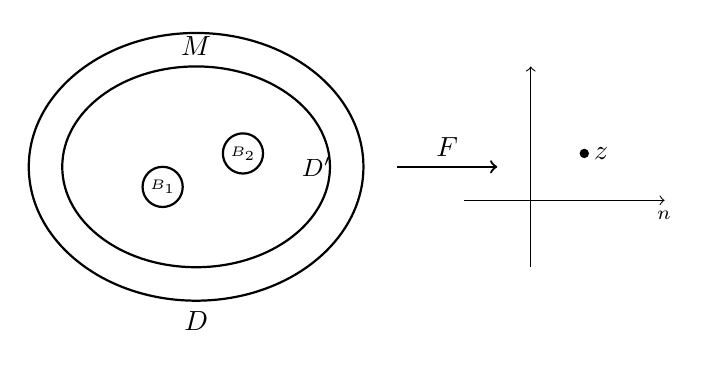
\begin{tikzpicture}[scale=0.85]
        % D' (D with balls removed)
        \draw[thick] (0,0) ellipse (2 and 1.5);
        \node at (0,1.8) {$M$};
        \draw[thick] (0,0) ellipse (2.5 and 2);
        \node at (0,-2.3) {$D$};
        % Small balls removed
        \draw[thick,fill=white] (-0.5,-0.3) circle (0.3);
        \node at (-0.5,-0.3) {\tiny $B_1$};
        \draw[thick,fill=white] (0.7,0.2) circle (0.3);
        \node at (0.7,0.2) {\tiny $B_2$};
        \node at (1.8,0) {\small $D'$};
        % Arrow
        \draw[->,thick] (3,0) -- (4.5,0) node[midway,above] {$F$};
        % R^n
        \draw[->] (5,-1.5) -- (5,1.5);
        \draw[->] (4,-0.5) -- (7,-0.5);
        \node at (7,-0.8) {$\R^n$};
        \fill (5.8,0.2) circle (2pt) node[right] {$z$};
    \end{tikzpicture}
    \end{center}
\end{proof}

\subsection{Jordan--Brouwer Separation Theorem}

When $M$ is a compact, connected hypersurface in $\R^n$ (i.e.\ codimension 1 submanifold), we can use the winding numbers to prove:

\begin{theorem}{Jordan--Brouwer Separation Theorem}{jordan-brouwer}
    The complement of a compact, connected hypersurface $M$ in $\R^n$ consists of two connected open sets, the ``outside'' $D_0$ and the ``inside'' $D_1$. Moreover, $\bar{D}_1$ is a compact $n$-manifold with boundary $\partial \bar{D}_1 = M$.
\end{theorem}

\begin{proof}[Proof sketch]
    Let $D_a := \{z \in \R^n \setminus M \mid \operatorname{wind}_{\Z/2}(M, z) = a\}$ for each $a \in \Z/2$, so that $\R^n \setminus M = D_0 \sqcup D_1$. Since $\operatorname{wind}_{\Z/2}(M, z)$ is locally constant, they are both open.

    For each $x \in M$, if $B$ is a small open ball around $x$ in $\R^n$, then $B \setminus M = B_0 \sqcup B_1$, where $B_0, B_1$ are two connected half balls, and $B_a = D_a \cap B$.

    \begin{center}
    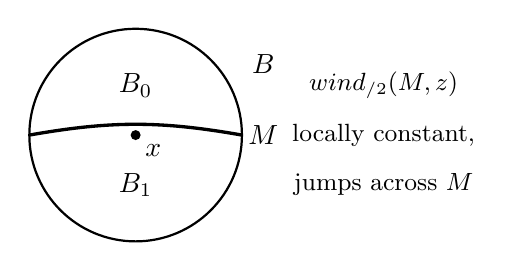
\begin{tikzpicture}[scale=0.9]
        % Ball B
        \draw[thick] (0,0) circle (1.5);
        \node at (1.8,1) {$B$};
        % M cutting through
        \draw[very thick] (-1.5,0) to[out=10,in=170] (1.5,0);
        \node at (1.8,0) {$M$};
        % Labels
        \node at (0,0.7) {$B_0$};
        \node at (0,-0.7) {$B_1$};
        \fill (0,0) circle (2pt) node[below right] {$x$};
        % Winding number annotation
        \node at (3.5,0.7) {\small $\operatorname{wind}_{\Z/2}(M,z)$};
        \node at (3.5,0) {\small locally constant,};
        \node at (3.5,-0.7) {\small jumps across $M$};
    \end{tikzpicture}
    \end{center}

    Connectivity of $M$ implies $D_a$ is connected, and compactness of $M$ implies $\bar{D}_1$ is compact.
\end{proof}

\section{Borsuk--Ulam Theorem}

\begin{theorem}{Borsuk--Ulam Theorem}{borsuk-ulam}
    Let $f \colon S^n \to \R^{n+1} \setminus \{0\}$ be a smooth map such that $f(-x) = -f(x)$ for all $x \in S^n$. Then $\operatorname{wind}_{\Z/2}(f, 0) = 1$.
\end{theorem}

\begin{proof}
    Let's proceed by induction on $n$.

    For $n = 1$, if $f \colon S^1 \to S^1$ is an antipodal map, then its lift $\tilde{f} \colon \R \to \R$ must satisfy $\tilde{f}(\theta + \pi) = \tilde{f}(\theta) + k\pi$ for some odd $k$, and $\deg_{\Z/2} f = k = 1 \pmod{2}$.

    Now assume the theorem for $n - 1$, and let $f \colon S^n \to \R^{n+1} \setminus \{0\}$ be antipodal. The idea is to compute $\operatorname{wind}_{\Z/2}(f, 0)$ by $I_2(f, R)$ for some ray $R$ from $0$.

    Let $g = f|_{S^{n-1}}$ (the equator $S^n \cap \{x_{n+1} = 0\}$) and use Sard to choose a unit vector $v$ that is a regular value for both $\frac{g}{|g|} \colon S^{n-1} \to S^n$ and $\frac{f}{|f|} \colon S^n \to S^n$.

    Let $\ell = \R \cdot v$ be the corresponding line. Then $f \pitchfork \ell$, and $g$ never intersects $\ell$.

    Now,
    \[
        \operatorname{wind}_{\Z/2}(f, 0) = \deg_{\Z/2}\!\left(\frac{f}{|f|}\right) = \#\left(\frac{f}{|f|}\right)^{-1}(v) \mod 2 = \frac{1}{2} \# f^{-1}(\ell) = \# f_+^{-1}(\ell) \mod 2,
    \]
    where $f_+ = f|_{S^n_+}$ is the restriction to the upper hemisphere.

    \begin{center}
    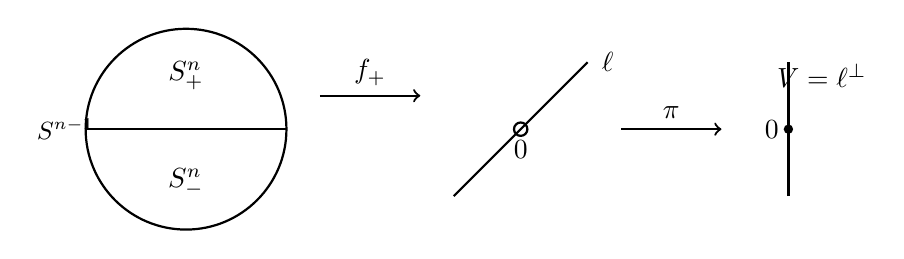
\begin{tikzpicture}[scale=0.85]
        % S^n (circle representation)
        \draw[thick] (0,0) circle (1.5);
        \draw[thick] (-1.5,0) -- (1.5,0);
        \node at (0,0.8) {$S^n_+$};
        \node at (0,-0.8) {$S^n_-$};
        \node at (-1.8,0) {\small $S^{n-1}$};
        % Arrow f_+
        \draw[->,thick] (2,0.5) -- (3.5,0.5) node[midway,above] {$f_+$};
        % Target with line l
        \draw[thick] (5,0) circle (0.1);
        \node at (5,-0.3) {$0$};
        \draw[thick] (4,-1) -- (6,1);
        \node at (6.3,1) {$\ell$};
        % Arrow pi
        \draw[->,thick] (6.5,0) -- (8,0) node[midway,above] {$\pi$};
        % V = l^perp
        \draw[thick] (9,-1) -- (9,1);
        \node at (9.5,0.8) {$V = \ell^\perp$};
        \fill (9,0) circle (2pt) node[left] {$0$};
    \end{tikzpicture}
    \end{center}

    By induction hypothesis,
    \[
        \operatorname{wind}_{\Z/2}(f, 0) = \# f_+^{-1}(\ell) = \#(\pi \circ f_+)^{-1}(0) = \operatorname{wind}_{\Z/2}\!\left(\pi \circ g, 0\right) = 1 \mod 2.
    \]
\end{proof}

\begin{corollary}{}{borsuk-ulam-cor1}
    If $f \colon S^n \to \R^{n+1} \setminus \{0\}$ is antipodal, then $f$ intersects every line through $0$ at least once.
\end{corollary}

\begin{corollary}{}{borsuk-ulam-cor2}
    For any $n$ smooth functions $g_1, \ldots, g_n$ on $S^n$, such that $g_i(p) = g_i(-p)$ for all $i = 1, \ldots, n$, there exists a point $p \in S^n$ at which all $g_i$ vanish simultaneously.
\end{corollary}

\begin{proof}
    If not, apply the corollary to the map $f(x) = (g_1(x) - g_1(-x), \ldots, g_n(x) - g_n(-x), 0)$ and take the $x_{n+1}$ axis for $\ell$.
\end{proof}


\chapter{Orientation}
% lecture14.tex — Orientation

\section{Orientation}

\begin{definition}{Equivalently Oriented Bases}{equiv-oriented-bases}
    Suppose $V$ is a finite dimensional real vector space, and $\beta = \{v_1, \ldots, v_k\}$ and $\beta' = \{v_1', \ldots, v_k'\}$ are two ordered bases. Then there is a unique linear isomorphism $A \colon V \to V$ such that $\beta' = A\beta$. We say $\beta$ and $\beta'$ are \emph{equivalently oriented} if $\det A > 0$.
\end{definition}

This gives an equivalence relation on the set of all ordered bases of $V$, and there are exactly two equivalence classes ($\operatorname{GL}(V)$ has 2 components).

\begin{definition}{Orientation of a Vector Space}{orientation-vector-space}
    An \emph{orientation} of $V$ is a choice of one of those two equivalence classes.
\end{definition}

An orientation induces a sign ($+$ or $-$) on any ordered basis of $V$.

($*$ When $V = 0$, we separately define its orientation to be a choice of a sign $\in \{+, -\}$.)

\begin{example}{Orientation of $\R^2$}{orientation-R2}
    Say, $V = \R^2$ and choose $[(e_1, e_2)]$ for the orientation. Then counterclockwise bases are positively oriented, while clockwise bases are negatively oriented.
\end{example}

\begin{center}
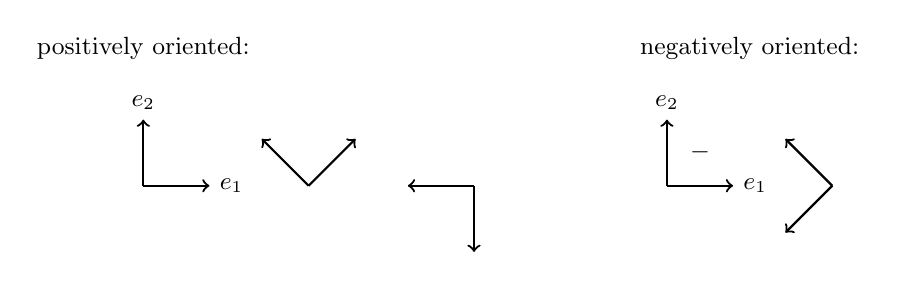
\begin{tikzpicture}[scale=0.7]
    % Positively oriented examples
    \node at (0,2.5) {\small positively oriented:};
    % Standard basis
    \draw[->,thick] (0,0) -- (1.2,0) node[right] {\small $e_1$};
    \draw[->,thick] (0,0) -- (0,1.2) node[above] {\small $e_2$};
    % Rotated
    \begin{scope}[xshift=3cm]
        \draw[->,thick] (0,0) -- (0.85,0.85);
        \draw[->,thick] (0,0) -- (-0.85,0.85);
    \end{scope}
    % Another
    \begin{scope}[xshift=6cm]
        \draw[->,thick] (0,0) -- (-1.2,0);
        \draw[->,thick] (0,0) -- (0,-1.2);
    \end{scope}
    % Negatively oriented examples
    \node at (11,2.5) {\small negatively oriented:};
    \begin{scope}[xshift=9.5cm]
        \draw[->,thick] (0,0) -- (0,1.2) node[above] {\small $e_2$};
        \draw[->,thick] (0,0) -- (1.2,0) node[right] {\small $e_1$};
        \node at (0.6,0.6) {\small $-$};
    \end{scope}
    \begin{scope}[xshift=12.5cm]
        \draw[->,thick] (0,0) -- (-0.85,0.85);
        \draw[->,thick] (0,0) -- (-0.85,-0.85);
    \end{scope}
\end{tikzpicture}
\end{center}

Note, if $V$ and $W$ are oriented real vector spaces of the same dimension, then any isomorphism $A \colon V \to W$ either \emph{preserves} or \emph{reverses} orientation.

\subsection{Orientation of Manifolds}

\begin{definition}{Orientation of a Manifold}{orientation-manifold}
    An \emph{orientation} of $M$, a manifold with boundary, is a smooth choice of orientations for all tangent spaces $T_p M$.

    That is, around each $p \in M$, there is a local parametrization $h \colon U \to M$, $U \subset H^m \subset \R^m$, such that $dh_u \colon T_u U \cong \R^m \to T_{h(u)} M$ preserves orientation for all $u \in U$, where $\R^m$ is given the standard orientation $[(e_1, \ldots, e_m)]$.
\end{definition}

A smooth map between oriented manifolds of the same dimension whose derivative preserves orientations at every point is called an \emph{orientation-preserving map}.

\begin{example}{Non-Orientable Manifolds}{non-orientable}
    Not all manifolds can be oriented! The M\"obius band is not orientable.
\end{example}

\begin{center}
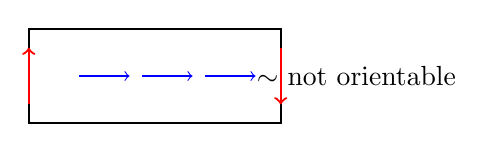
\begin{tikzpicture}[scale=0.8]
    % Mobius band as rectangle with identification
    \draw[thick] (0,0) rectangle (4,1.5);
    % Arrows on left side (upward)
    \draw[->,thick,red] (0,0.3) -- (0,1.2);
    % Arrows on right side (downward — reversed!)
    \draw[->,thick,red] (4,1.2) -- (4,0.3);
    % Orientation arrows along the band
    \draw[->,blue] (0.8,0.75) -- (1.6,0.75);
    \draw[->,blue] (1.8,0.75) -- (2.6,0.75);
    \draw[->,blue] (2.8,0.75) -- (3.6,0.75);
    \node at (5.2,0.75) {$\sim$ not orientable};
\end{tikzpicture}
\end{center}

\begin{example}{Orientable Manifolds}{orientable-examples}
    $T^2$ (torus) and $S^2$ (sphere) are orientable.
\end{example}

\begin{center}
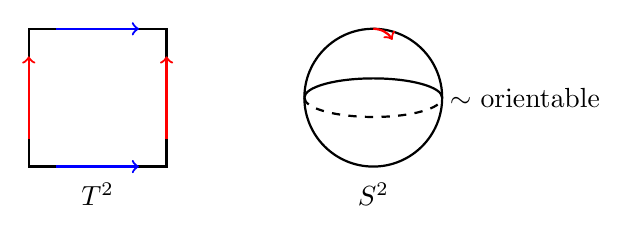
\begin{tikzpicture}[scale=0.7]
    % Torus as rectangle with identifications
    \draw[thick] (0,0) rectangle (2.5,2.5);
    \draw[->,thick,red] (0,0.5) -- (0,2);
    \draw[->,thick,red] (2.5,0.5) -- (2.5,2);
    \draw[->,thick,blue] (0.5,0) -- (2,0);
    \draw[->,thick,blue] (0.5,2.5) -- (2,2.5);
    \node at (1.25,-0.5) {$T^2$};
    % Sphere
    \begin{scope}[xshift=5cm]
        \draw[thick] (1.25,1.25) circle (1.25);
        \draw[thick,dashed] (0,1.25) arc(180:360:1.25 and 0.35);
        \draw[thick] (0,1.25) arc(180:0:1.25 and 0.35);
        % Orientation arrow
        \draw[->,thick,red] (1.25,2.5) arc(90:30:0.4);
        \node at (1.25,-0.5) {$S^2$};
    \end{scope}
    \node at (9,1.25) {$\sim$ orientable};
\end{tikzpicture}
\end{center}

\begin{proposition}{Two Orientations}{two-orientations}
    A connected, orientable manifold with boundary admits exactly two orientations.
\end{proposition}

\begin{proof}
    The set of points at which two orientations agree and the set where they disagree are both open. Consequently, two orientations of a connected manifold are either identical or opposite.
\end{proof}

\subsection{Product and Boundary Orientations}

\begin{remark}{Product and Boundary Orientations}{product-boundary-orientations}
    \begin{itemize}
        \item The product $M \times N$ of two oriented manifolds (where one of them is boundaryless) acquires a \emph{product orientation}, for if $\alpha$ and $\beta$ are ordered bases for $T_p M$ and $T_q N$, then $(\alpha \times 0, 0 \times \beta)$ is an ordered basis for $T_{(p,q)}(M \times N) \cong T_p M \times T_q N$.

        \item An orientation of $M$ induces a \emph{boundary orientation} on $\partial M$; this can be done by declaring the sign of any ordered basis $\beta = \{v_1, \ldots, v_{m-1}\}$ of $T_p(\partial M)$ to be the sign of the ordered basis $\{n_p, v_1, \ldots, v_{m-1}\}$, where $n_p$ is the outward unit normal at $p$.
    \end{itemize}
\end{remark}

\begin{example}{Boundary Orientation of $I \times M$}{boundary-orientation-cylinder}
    For the cylinder $I \times M$, the boundary orientation gives $\partial(I \times M) = M_1 - M_0$, where $M_0$ and $M_1$ have opposite orientations.
\end{example}

\begin{center}
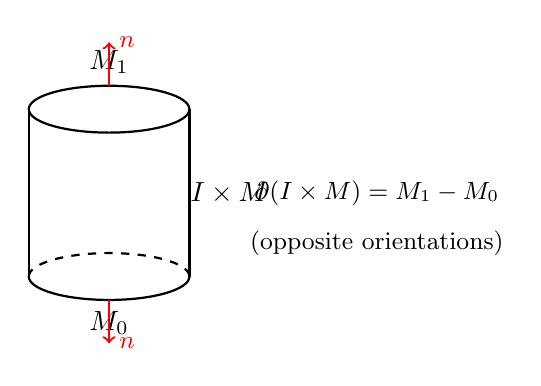
\begin{tikzpicture}[scale=0.85]
    % Cylinder
    \draw[thick] (-1.2,0) -- (-1.2,2.5);
    \draw[thick] (1.2,0) -- (1.2,2.5);
    % Bottom circle M_0
    \draw[thick] (-1.2,0) arc(180:360:1.2 and 0.35);
    \draw[thick,dashed] (-1.2,0) arc(180:0:1.2 and 0.35);
    % Top circle M_1
    \draw[thick] (-1.2,2.5) arc(180:360:1.2 and 0.35);
    \draw[thick] (-1.2,2.5) arc(180:0:1.2 and 0.35);
    % Labels
    \node at (0,-0.7) {$M_0$};
    \node at (0,3.2) {$M_1$};
    \node at (1.8,1.25) {$I \times M$};
    % Outward normals
    \draw[->,thick,red] (0,2.85) -- (0,3.5) node[right] {\small $n$};
    \draw[->,thick,red] (0,-0.35) -- (0,-1) node[right] {\small $n$};
    % Orientation note
    \node at (4,1.25) {\small $\partial(I \times M) = M_1 - M_0$};
    \node at (4,0.5) {\small (opposite orientations)};
\end{tikzpicture}
\end{center}

\subsection{Orienting Preimages}

If $V = V_1 \oplus V_2$, the orientations on any two of $V$, $V_1$, $V_2$ induce a \emph{direct sum orientation} on the third. (The ordering of summands is important!)

We can use this to orient $f^{-1}(P) =: Q$ if $f \colon M \to N$, $f \pitchfork P$, $f|_{\partial M} \pitchfork P$, and $M$, $N$, $P$ are all oriented.

Let $N_x(Q; M)$ be the orthogonal complement of $T_x Q$ in $T_x M$, so that
\[
    T_x M = N_x(Q; M) \oplus T_x Q.
\]
By transversality,
\[
    T_y N = df_x(N_x(Q; M)) \oplus T_y P,
\]
which gives an orientation on $T_x Q$!

\begin{proposition}{Boundary of Preimage}{boundary-preimage-orientation}
    $\partial f^{-1}(P) = (-1)^{\codim P} (f|_{\partial M})^{-1}(P)$.
\end{proposition}

\begin{proof}[Proof sketch]
    $T_x M = N_x(Q; M) \oplus \R \cdot n_x \oplus T_x(\partial Q) = \R \cdot n_x \oplus N_x(Q; M) \oplus T_x((f|_{\partial M})^{-1}(P))$, so the orientations differ by $(-1)^{\codim Q} = (-1)^{\codim P}$.
\end{proof}


\chapter{Oriented Intersection Number}
% lecture15.tex — Oriented Intersection Number

\section{Oriented Intersection Number}

Consider oriented manifolds $M, N, P$, with $M$ compact, $P \subset N$ closed, and
\[
    \dim M + \dim P = \dim N.
\]

If $f \colon M \to N$ is transversal to $P$, then $f^{-1}(P)$ is a finite number of points, each with an orientation number $\in \{\pm 1\}$.

\begin{definition}{Intersection Number}{intersection-number}
    The \emph{intersection number} $I(f, P) \in \Z$ is defined to be the sum of these orientation numbers.
\end{definition}

The orientation number at $x \in f^{-1}(P)$ is $+1$ (resp.\ $-1$) if the isomorphism
\[
    df_x(T_x M) \oplus T_{f(x)} P = T_{f(x)} N
\]
is orientation preserving (resp.\ reversing). Note, the ordering is important!

\begin{example}{Circles on a Torus}{torus-circles}
    For the two standard circles $C_1, C_2$ on a torus, $I(C_1, C_2) = 1$ and $I(C_2, C_1) = -1$.
\end{example}

\begin{center}
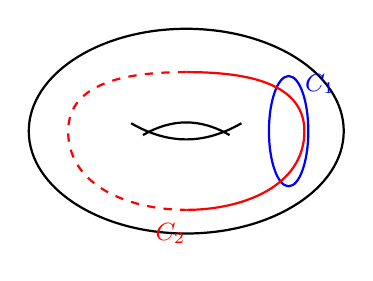
\begin{tikzpicture}[scale=1]
    % Torus outline
    \draw[thick] (0,0) ellipse (2 and 1.3);
    % Inner hole
    \draw[thick] (-0.7,0.1) to[out=-30,in=210] (0.7,0.1);
    \draw[thick] (-0.55,-0.05) to[out=30,in=150] (0.55,-0.05);
    % Meridian C_1 (goes around the tube)
    \draw[thick,blue] (1.3,0) ellipse (0.25 and 0.7);
    \node[blue] at (1.7,0.6) {\small $C_1$};
    % Longitude C_2 (goes around the hole)
    \draw[thick,red] (0,-1.0) to[out=0,in=-90] (1.5,0) to[out=90,in=0] (0,0.75);
    \draw[thick,red,dashed] (0,0.75) to[out=180,in=90] (-1.5,0) to[out=-90,in=180] (0,-1.0);
    \node[red] at (-0.2,-1.3) {\small $C_2$};
\end{tikzpicture}
\end{center}

\begin{proposition}{Vanishing on Boundaries}{intersection-boundary-zero}
    If $M = \partial W$ for some compact, oriented $W$ and $f \colon M \to N$ extends to $W$, then $I(f, P) = 0$ for any closed $P \subset N$ of complementary dimension.
\end{proposition}

\begin{proof}
    The proof is the same as the analogous theorem in mod 2 intersection theory. Here, $F^{-1}(P)$ is a compact oriented 1-manifold, so the signed count of $\partial F^{-1}(P)$ is $0$.
\end{proof}

\begin{center}
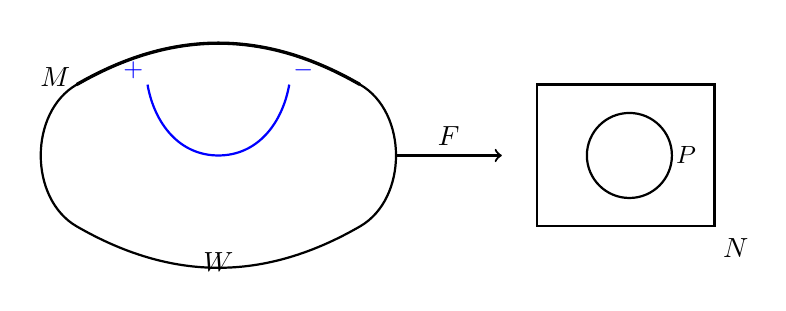
\begin{tikzpicture}[scale=0.9]
    % W (blob) with M = boundary
    \draw[thick] (0,0) to[out=30,in=150] (4,0) to[out=-30,in=30] (4,-2) to[out=210,in=330] (0,-2) to[out=150,in=210] cycle;
    \node at (2,-2.5) {$W$};
    \draw[very thick] (0,0) to[out=30,in=150] (4,0);
    \node at (-0.3,0.1) {$M$};
    % F^{-1}(P) arc with signed endpoints
    \draw[thick,blue] (1,0) to[out=-80,in=180] (2,-1) to[out=0,in=260] (3,0);
    \node[blue] at (0.8,0.2) {\small $+$};
    \node[blue] at (3.2,0.2) {\small $-$};
    % Arrow + F label to right
    \draw[->,thick] (4.5,-1) -- (6,-1) node[midway,above] {$F$};
    % N with P inside
    \draw[thick] (6.5,-2) rectangle (9,0);
    \node at (9.3,-2.3) {$N$};
    \draw[thick] (7.8,-1) circle (0.6);
    \node at (8.6,-1) {\small $P$};
\end{tikzpicture}
\end{center}

\begin{proposition}{Homotopy Invariance}{intersection-homotopy}
    Homotopic maps have the same intersection numbers.
\end{proposition}

\begin{proof}
    The proof is analogous to the mod 2 case. If $F \colon I \times M \to N$ is a homotopy between $f_0, f_1 \colon M \to N$, then
    \[
        0 = I(\partial F, P) = I(f_1, P) - I(f_0, P),
    \]
    since $\partial(I \times M) = M_1 - M_0$, so $\partial F^{-1}(P) = f_1^{-1}(P) - f_0^{-1}(P)$.
\end{proof}

\subsection{Degree}

In the same manner, when $N$ is connected and $\dim N = \dim M$, we define the \emph{degree} of $f \colon M \to N$ to be
\[
    \deg(f) = I(f, \{y\}),
\]
for any (positively oriented) point $y \in N$.

\begin{example}{Winding Number}{winding-number}
    The winding number of a closed curve in the plane around a point is a degree.
\end{example}

\begin{center}
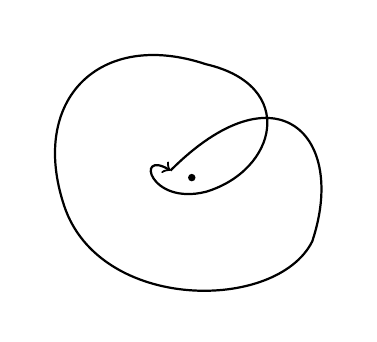
\begin{tikzpicture}[scale=0.9]
    % A closed curve winding around a point
    \draw[thick,->] (0,0) .. controls (1.5,1.5) and (2.5,0.5) .. (2,-1)
        .. controls (1.5,-2) and (-1,-2) .. (-1.5,-0.5)
        .. controls (-2,1) and (-1,2) .. (0.5,1.5)
        .. controls (1.8,1.2) and (1.5,0) .. (0.5,-0.3)
        .. controls (-0.3,-0.5) and (-0.5,0.3) .. (0,0);
    \fill (0.3,-0.1) circle (1.5pt);
\end{tikzpicture}
\end{center}

\begin{example}{Degree of $z \mapsto z^m$}{degree-power}
    The map $S^1 \to S^1$, $z \mapsto z^m$, has degree $m \in \Z$. In particular, $z^m$ and $z^{m'}$ (as maps $S^1 \to S^1$) are not homotopic whenever $m \neq m'$.
\end{example}

\subsection{Reformulation via the Diagonal}

The following reformulation is useful.

Let $M_1, M_2$ be compact with $\dim M_1 + \dim M_2 = \dim N$. For any $f_1 \colon M_1 \to N$ and $f_2 \colon M_2 \to N$, we say they are \emph{transversal}, $f_1 \pitchfork f_2$, if
\begin{equation}
    (df_1)_{x_1}(T_{x_1} M_1) \oplus (df_2)_{x_2}(T_{x_2} M_2) = T_y N \tag{$*$}
\end{equation}
whenever $f_1(x_1) = y = f_2(x_2)$.

Basic linear algebra shows $f_1 \pitchfork f_2 \iff f_1 \times f_2 \pitchfork \Delta$, where $f_1 \times f_2 \colon M_1 \times M_2 \to N \times N$ and $\Delta \subset N \times N$ is the \emph{diagonal}.

Define $I(f_1, f_2)$ to be the sum of local intersection numbers, each of which is given by $+1$ (resp.\ $-1$) if the isomorphism ($*$) is orientation preserving (resp.\ reversing).

\begin{proposition}{Intersection via Diagonal}{intersection-diagonal}
    \[
        I(f_1, f_2) = (-1)^{\dim(M_2)} \, I(f_1 \times f_2, \Delta).
    \]
\end{proposition}

\begin{proof}
    This is linear algebra again. Let $U = (df_1)_{x_1}(T_{x_1} M_1)$ and $V = (df_2)_{x_2}(T_{x_2} M_2)$, and let $\{u_1, \ldots, u_k\}$ and $\{v_1, \ldots, v_\ell\}$ be their positively oriented ordered bases. We may assume $\{u_1, \ldots, u_k, v_1, \ldots, v_\ell\}$ is positively oriented for $T_y N$. Then, for $U \times V$,
    \begin{align*}
        &\sign\{(u_1, 0), \ldots, (u_k, 0), (0, v_1), \ldots, (0, v_\ell), (u_1, u_1), \ldots, (u_k, u_k), (v_1, v_1), \ldots, (v_\ell, v_\ell)\} \\
        &\qquad = \sign\{(u_1, 0), \ldots, (u_k, 0), (0, v_1), \ldots, (0, v_\ell), (0, u_1), \ldots, (0, u_k), (v_1, 0), \ldots, (v_\ell, 0)\} \\
        &\qquad = (-1)^{\ell(\ell + k) + \ell k} \sign\{(u_1, 0), \ldots, (v_\ell, 0), (0, u_1), \ldots, (0, v_\ell)\} \\
        &\qquad = (-1)^\ell.
    \end{align*}
\end{proof}

\begin{proposition}{Homotopy Invariance of Pairs}{intersection-pairs-homotopy}
    If $f_0$ and $g_0$ are homotopic to $f_1$ and $g_1$, respectively, then $I(f_0, g_0) = I(f_1, g_1)$.
\end{proposition}

\begin{proof}
    $f_t \times g_t$ is a homotopy between $f_0 \times g_0$ and $f_1 \times g_1$.
\end{proof}

In particular, if $M_1, M_2 \subset N$ are compact submanifolds of complementary dimension, then $I(M_1, M_2)$ is invariant under homotopy of either $M_1$ or $M_2$.

Note, from the definition,
\[
    I(M_1, M_2) = (-1)^{(\dim M_1)(\dim M_2)} I(M_2, M_1).
\]

\subsection{Euler Characteristic}

\begin{definition}{Euler Characteristic}{euler-characteristic}
    If $M$ is a compact, orientable manifold, its \emph{Euler characteristic} $\chi(M)$ is defined to be $I(\Delta, \Delta)$, where $\Delta \subset M \times M$ is the diagonal.
\end{definition}

We immediately have:

\begin{proposition}{Odd-Dimensional Euler Characteristic}{odd-dim-euler}
    The self-intersection number of any odd-dimensional compact oriented manifold is $0$. In particular, $\chi(M) = 0$ for any odd-dimensional compact oriented manifold.
\end{proposition}

Recall that $I_{\Z/2}(C, C) = 1$ for the central circle $C$ in the M\"obius strip. This shows that the M\"obius strip is \emph{not orientable} (for if it were, then $I_{\Z/2}(C, C) = I(C, C) \mod 2 = 0$).


\chapter{Lefschetz Fixed Point Theorem}
% lecture16.tex — Lefschetz Fixed Point Theorem

\section{Lefschetz Fixed Point Theorem}

Let $M$ be a compact, oriented manifold, and $f \colon M \to M$ a smooth map.

\begin{definition}{Global Lefschetz Number}{global-lefschetz}
    The \emph{global Lefschetz number} of $f$, denoted $L(f)$, is
    \[
        L(f) = I(\Delta, \operatorname{graph}(f)).
    \]
\end{definition}

The following are immediate consequences of the intersection theory. Note that fixed points of $f$ correspond exactly to intersection points $\Delta \cap \operatorname{graph}(f)$.

\begin{proposition}{Homotopy Invariance of $L$}{lefschetz-homotopy}
    $L(f)$ is a homotopy invariant.
\end{proposition}

\begin{theorem}{Smooth Lefschetz Fixed Point Theorem}{lefschetz-fixed-point}
    If $L(f) \neq 0$, then $f$ has a fixed point.
\end{theorem}

\begin{proposition}{Lefschetz Number of Identity}{lefschetz-identity}
    If $f$ is homotopic to the identity, then $L(f) = \chi(M)$.
\end{proposition}

In particular, if $M$ admits a smooth map $f \colon M \to M$ homotopic to the identity that has no fixed points, then $\chi(M) = 0$.

\begin{example}{Euler Characteristic of $S^1$}{euler-S1}
    Rotation of $S^1$ by an angle $\theta \neq 0 \mod 2\pi$ has no fixed points, so $\chi(S^1) = 0$.
\end{example}

\subsection{Lefschetz Maps and Local Lefschetz Numbers}

\begin{definition}{Lefschetz Map}{lefschetz-map}
    We say a map $f \colon M \to M$ is \emph{Lefschetz} if $\Delta \pitchfork \operatorname{graph}(f)$.
\end{definition}

\begin{proposition}{Homotopy to Lefschetz}{homotopic-to-lefschetz}
    Every map $f \colon M \to M$ is homotopic to a Lefschetz map.
\end{proposition}

Note, $\Delta \pitchfork \operatorname{graph}(f)$ at $(x, x)$ iff
\begin{align*}
    \Delta_x + \operatorname{graph}(df_x) &= T_x M \times T_x M \\
    &\iff \Delta_x \cap \operatorname{graph}(df_x) = 0 \\
    &\iff df_x \text{ has no eigenvector of eigenvalue } 1 \\
    &\iff \det(df_x - I) \neq 0.
\end{align*}

\begin{definition}{Lefschetz Fixed Point}{lefschetz-fixed-pt}
    A fixed point $x$ of $f$ is a \emph{Lefschetz fixed point} if $\det(df_x - I) \neq 0$.
\end{definition}

\begin{definition}{Local Lefschetz Number}{local-lefschetz}
    For a Lefschetz fixed point $x$ of $f$, the \emph{local Lefschetz number} of $f$ at $x$, $L_x(f)$, is the orientation number $\in \{\pm 1\}$ of $(x, x) \in \Delta \cap \operatorname{graph}(f)$.
\end{definition}

Clearly, for Lefschetz maps,
\[
    L(f) = \sum_{f(x) = x} L_x(f),
\]
the sum being over fixed points.

\begin{proposition}{Formula for Local Lefschetz Number}{local-lefschetz-formula}
    \[
        L_x(f) = \sign(\det(df_x - I)).
    \]
\end{proposition}

\begin{proof}
    The proof is simple linear algebra. If $\{v_1, \ldots, v_m\}$ is a positively oriented ordered basis for $T_x M$, then
    \begin{align*}
        L_x(f) &= \sign\{\underbrace{(v_1, v_1), \ldots, (v_m, v_m)}_{\text{positive for } T_{(x,x)}\Delta}, \underbrace{(v_1, df_x(v_1)), \ldots, (v_m, df_x(v_m))}_{\text{positive for } T_{(x,x)} \operatorname{graph}(f)}\} \\
        &= \sign\{(v_1, v_1), \ldots, (v_m, v_m), (0, (df_x - I)v_1), \ldots, (0, (df_x - I)v_m)\} \\
        &= \sign\{(v_1, 0), \ldots, (v_m, 0), (0, (df_x - I)v_1), \ldots, (0, (df_x - I)v_m)\} \\
        &= \sign(\det(df_x - I)).
    \end{align*}
\end{proof}

\subsection{Local Pictures in 2D}

\begin{example}{Local Pictures in 2D}{local-pictures-2d}
    Assume that $df_x = \begin{pmatrix} \alpha_1 & 0 \\ 0 & \alpha_2 \end{pmatrix}$ with $\alpha_1, \alpha_2 > 0$.

    \textbf{Case 1:} If either $\alpha_1, \alpha_2 > 1$ or $\alpha_1, \alpha_2 < 1$, then $L_x(f) = +1$ (source or sink).

    \textbf{Case 2:} If $\alpha_1 < 1 < \alpha_2$, then $L_x(f) = -1$ (saddle).
\end{example}

\begin{center}
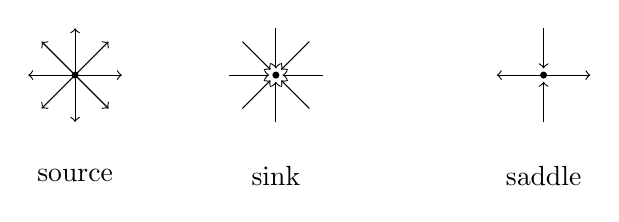
\begin{tikzpicture}[scale=0.85]
    % Source
    \node at (0,-1.5) {source};
    \fill (0,0) circle (1.5pt);
    \draw[->] (0,0) -- (0.7,0);
    \draw[->] (0,0) -- (-0.7,0);
    \draw[->] (0,0) -- (0,0.7);
    \draw[->] (0,0) -- (0,-0.7);
    \draw[->] (0,0) -- (0.5,0.5);
    \draw[->] (0,0) -- (-0.5,0.5);
    \draw[->] (0,0) -- (0.5,-0.5);
    \draw[->] (0,0) -- (-0.5,-0.5);
    % Sink
    \begin{scope}[xshift=3cm]
        \node at (0,-1.5) {sink};
        \fill (0,0) circle (1.5pt);
        \draw[->] (0.7,0) -- (0.1,0);
        \draw[->] (-0.7,0) -- (-0.1,0);
        \draw[->] (0,0.7) -- (0,0.1);
        \draw[->] (0,-0.7) -- (0,-0.1);
        \draw[->] (0.5,0.5) -- (0.08,0.08);
        \draw[->] (-0.5,0.5) -- (-0.08,0.08);
        \draw[->] (0.5,-0.5) -- (0.08,-0.08);
        \draw[->] (-0.5,-0.5) -- (-0.08,-0.08);
    \end{scope}
    % Saddle
    \begin{scope}[xshift=7cm]
        \node at (0,-1.5) {saddle};
        \fill (0,0) circle (1.5pt);
        % In along y, out along x
        \draw[->] (0,0.7) -- (0,0.1);
        \draw[->] (0,-0.7) -- (0,-0.1);
        \draw[->] (0,0) -- (0.7,0);
        \draw[->] (0,0) -- (-0.7,0);
    \end{scope}
\end{tikzpicture}
\end{center}

\subsection{Euler Characteristic from Local Lefschetz Numbers}

\begin{example}{Euler Characteristic of $S^2$}{euler-S2-downward-flow}
    Consider the map $f_t \colon S^2 \to S^2$ given by a ``downward flow''
    \[
        f_t(x) = \pi\!\left(x + \left(0, 0, -\tfrac{t}{2}\right)\right), \quad 0 < t < 2,
    \]
    where $\pi \colon \R^3 \setminus \{0\} \to S^2$ is the projection. This has a source at the north pole and a sink at the south pole, giving
    \[
        \chi(S^2) = L(f_1) = 1 + 1 = 2.
    \]
\end{example}

\begin{center}
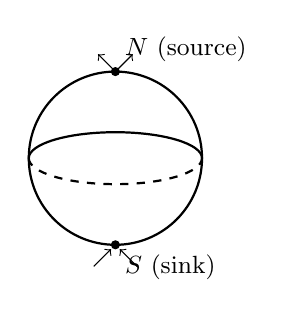
\begin{tikzpicture}[scale=1.1]
    % Sphere
    \draw[thick] (0,0) circle (1);
    \draw[thick,dashed] (-1,0) arc(180:360:1 and 0.3);
    \draw[thick] (-1,0) arc(180:0:1 and 0.3);
    % North pole (source)
    \fill (0,1) circle (1.5pt);
    \node[above right] at (0,1) {\small $N$ (source)};
    \draw[->] (0,1) -- (0.2,1.2);
    \draw[->] (0,1) -- (-0.2,1.2);
    % South pole (sink)
    \fill (0,-1) circle (1.5pt);
    \node[below right] at (0,-1) {\small $S$ (sink)};
    \draw[->] (0.25,-1.25) -- (0.05,-1.05);
    \draw[->] (-0.25,-1.25) -- (-0.05,-1.05);
\end{tikzpicture}
\end{center}

\begin{corollary}{Fixed Points of Maps on $S^2$}{s2-fixed-point}
    Every map $f \colon S^2 \to S^2$ homotopic to the identity must have a fixed point. In particular, the antipodal map $x \mapsto -x$ is not homotopic to the identity.
\end{corollary}

More generally, a genus $g$ surface admits a Lefschetz map homotopic to the identity that has $1$ source, $1$ sink, and $2g$ saddles, giving
\[
    \chi(\Sigma_g) = 2 - 2g.
\]

It is also instructive to see how the fixed points get created and annihilated in pairs when we deform the ``height function''; for example, on $S^2$,
\[
    \chi(S^2) = 1 + 1 = 1 + 1 + (1 - 1).
\]


\chapter{Vector Fields and the Poincar\'e--Hopf Theorem}
% lecture17.tex — Vector Fields and the Poincaré–Hopf Theorem

\section{Vector Fields and the Poincar\'e--Hopf Theorem}

\begin{definition}{Vector Field}{vector-field}
    A \emph{vector field} on a manifold $M$ is a smooth section $v \colon M \to TM$, i.e.\ a smooth assignment of a tangent vector $v(x) \in T_x M$ at each point $x \in M$.
\end{definition}

If $v(x) \neq 0$ at some point $x \in M$, then $v$ is nearly constant in magnitude and direction near $x$.

\begin{center}
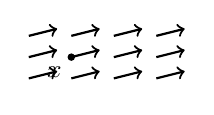
\begin{tikzpicture}[scale=0.9]
    \foreach \y in {-0.3, 0, 0.3} {
        \foreach \x in {-0.6, 0, 0.6, 1.2} {
            \draw[->,thick] (\x,\y) -- (\x+0.4,\y+0.1);
        }
    }
    \fill (0,0) circle (1.5pt) node[below left] {\small $x$};
\end{tikzpicture}
\end{center}

However, if $v(x) = 0$, $v$ can behave interestingly around such \emph{zeros}.

\begin{example}{Behaviors of Vector Fields Near Zeros}{vf-behaviors}
    On a surface, some possible behaviors of $v$ around its zeros include: sink, source, circulation, spiral, and saddle.
\end{example}

\begin{center}
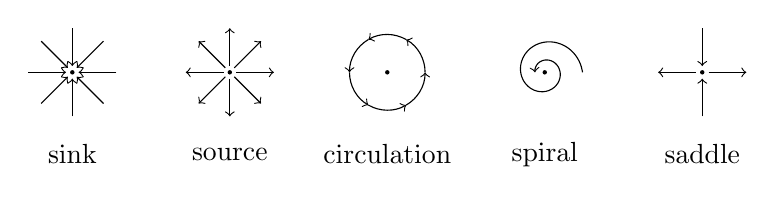
\begin{tikzpicture}[scale=0.8]
    % Sink
    \node at (0,-1.3) {sink};
    \fill (0,0) circle (1pt);
    \foreach \a in {0,45,90,135,180,225,270,315} {
        \draw[->] ({0.7*cos(\a)},{0.7*sin(\a)}) -- ({0.1*cos(\a)},{0.1*sin(\a)});
    }
    % Source
    \begin{scope}[xshift=2.5cm]
        \node at (0,-1.3) {source};
        \fill (0,0) circle (1pt);
        \foreach \a in {0,45,90,135,180,225,270,315} {
            \draw[->] ({0.1*cos(\a)},{0.1*sin(\a)}) -- ({0.7*cos(\a)},{0.7*sin(\a)});
        }
    \end{scope}
    % Circulation
    \begin{scope}[xshift=5cm]
        \node at (0,-1.3) {circulation};
        \fill (0,0) circle (1pt);
        \draw[->] (0.6,0) arc(0:60:0.6);
        \draw[->] (0.3,0.52) arc(60:120:0.6);
        \draw[->] (-0.3,0.52) arc(120:180:0.6);
        \draw[->] (-0.6,0) arc(180:240:0.6);
        \draw[->] (-0.3,-0.52) arc(240:300:0.6);
        \draw[->] (0.3,-0.52) arc(300:360:0.6);
    \end{scope}
    % Spiral
    \begin{scope}[xshift=7.5cm]
        \node at (0,-1.3) {spiral};
        \fill (0,0) circle (1pt);
        \draw[->,domain=0:540,smooth,variable=\t,samples=60]
            plot ({0.6*exp(-\t/400)*cos(\t)},{0.6*exp(-\t/400)*sin(\t)});
    \end{scope}
    % Saddle
    \begin{scope}[xshift=10cm]
        \node at (0,-1.3) {saddle};
        \fill (0,0) circle (1pt);
        \draw[->] (0,0.7) -- (0,0.1);
        \draw[->] (0,-0.7) -- (0,-0.1);
        \draw[->] (0.1,0) -- (0.7,0);
        \draw[->] (-0.1,0) -- (-0.7,0);
    \end{scope}
\end{tikzpicture}
\end{center}

We'll see that the zeros of $v$ encode some information on the topology of the manifold $M$!

\subsection{Index of a Vector Field}

Suppose $v$ is a vector field on $\R^m$ that has an isolated zero at the origin $0 \in \R^m$. Then, for any small enough radius $\varepsilon > 0$, $v$ has no zeros except at the origin inside the sphere $S_\varepsilon^{m-1}$ of radius $\varepsilon$ around the origin.

\begin{definition}{Index of a Vector Field at a Zero}{index-vf}
    The \emph{index} of $v$ at $0$, $\ind_0(v)$, is the degree of the directional map
    \[
        S_\varepsilon^{m-1} \to S^{m-1}, \quad x \mapsto \frac{v(x)}{|v(x)|}.
    \]
\end{definition}

\begin{example}{Index in Two Dimensions}{index-2d}
    In the two-dimensional case, $\ind_x(v)$ simply counts the number of times $v$ rotates (in the counterclockwise direction) as we walk counterclockwise around the circle. For example, a sink, source, circulation, and spiral each have index $+1$; a saddle has index $-1$; and a ``double rotation'' has index $+2$.
\end{example}

More generally, if $x$ is an isolated zero of a vector field $v$ on $M$, then we can define $\ind_x(v)$ to be the index of the pushforward vector field $\varphi_*^{-1}(v)$ at $0$, where $\varphi \colon U \to M$, $0 \mapsto x$, is a local parametrization.

\subsection{Poincar\'e--Hopf Theorem}

\begin{theorem}{Poincar\'e--Hopf Index Theorem}{poincare-hopf}
    If $v$ is a smooth vector field on a compact, oriented manifold $M$ with only finitely many zeros, then
    \[
        \chi(M) = \sum_{v(x) = 0} \ind_x(v).
    \]
\end{theorem}

\begin{corollary}{Hairy Ball Theorem}{hairy-ball}
    There is no nowhere-vanishing vector field on $S^2$, since $\chi(S^2) = 2 \neq 0$.

    ``You can't comb a hairy ball without leaving a bald spot.''
\end{corollary}

\begin{proof}[Proof of Poincar\'e--Hopf]
    The idea is that a vector field determines a flow
    \[
        f_t \colon M \to M
    \]
    that is homotopic to $f_0 = \id$, and tangent to $v$ at time zero. Such a family of maps can be obtained by solving the ODE given by the vector field. Another way is to simply take $f_t(x) = \pi(x + t v(x))$, where $\pi$ is the projection map from the $\varepsilon$-neighborhood theorem.

    For small $t > 0$, fixed points of $f_t$ correspond exactly to zeros of $v$, so it suffices to prove that $\ind_x(v) = L_x(f_t)$.

    This is a local problem, so we may work in $\R^m$. From basic calculus, there is a smooth vector-valued function $r(t, x)$ such that
    \[
        f_t(x) = f_0(x) + t f_0'(x) + t^2 r(t, x) = f_0(x) + t v(x) + t^2 r(t, x),
    \]
    so
    \[
        \frac{f_t(x) - x}{|f_t(x) - x|} = \frac{v(x) + t r(t, x)}{|v(x) + t r(t, x)|} \colon S_\varepsilon^{m-1} \to S^{m-1}
    \]
    is homotopic to $v(x)/|v(x)|$, whose degree is $\ind(v)$.

    On the other hand, the local Lefschetz number $L_x(f_t)$ is the degree of the map
    \[
        \partial B_\varepsilon^m \to S^{m-1}, \quad z \mapsto \frac{f_t(z) - z}{|f_t(z) - z|}.
    \]
    For Lefschetz fixed points, simple linear algebra shows that this agrees with the previous definition, since $\deg\!\left(z \mapsto \frac{(A - I)z}{|(A - I)z|}\right) = \sign \det(A - I)$.

    Homotopy invariance follows from the boundary theorem.
\end{proof}

\begin{corollary}{Euler Characteristic via Self-Intersection}{euler-self-intersection}
    $\chi(M) = I(M, M)$, where $M$ is considered as the $0$-section $M \subset TM$.
\end{corollary}


\end{document}
